\documentclass[a4paper,english]{report} 

\usepackage{fullpage}
\usepackage{subfig}
\usepackage[usenames,dvipsnames]{color}

\def\documentstate{final} % Lav om til FINAL når vi er done!
\usepackage[utf8]{inputenc}
\usepackage[\documentstate]{fixme} % kræver at folk er smarte nok til at installere FiXme
\usepackage[T1]{fontenc}
\usepackage{babel}
%\usepackage{lmodern} % vector font, ikke bitmap!!
% ^- kun interessant med latex, pdflatex er vector i forvejen
\usepackage[final]{graphicx}
\graphicspath{{graphics/}}
\DeclareGraphicsExtensions{.pdf,.jpeg,.jpg,.png}
\usepackage{tikz}
\usetikzlibrary{positioning,shadows,arrows}

\usepackage{caption}
\captionsetup{labelfont=bf, font=small}

\usepackage[final,plainpages=false]{hyperref}
\usepackage[final,english]{varioref}
\hypersetup{pdfborder=0 0 0} % Go away you ugly boxes!

\usepackage{amssymb}
\usepackage{amsmath}
\usepackage{verbatim}
\usepackage{multirow}
\usepackage{rotating}
\usepackage{listings}
\usepackage{listing}
\usepackage{algorithm}
\usepackage{algorithmic}
\usepackage[numbers]{natbib}

%\citestyle{chicago} % Chicago Manual of Style citations

\newcommand{\lookOfDisapproval}{
  \ensuremath{\overset{-\mkern-11mu-\mkern-3.5mu\rhook}{\smash{\odot}\rule{0ex}{.46ex}}\underline{\hspace{0.5em}}\overset{-\mkern-11mu-\mkern-3.5mu\rhook}{\smash{\odot}\rule{0ex}{.46ex}}}
}

%\renewcommand{\danishhyphenmins}{22} % fuck lorte orddeling!
\usepackage[\documentstate]{ifdraft}
\ifdraft{
  \usepackage{draftwatermark}
  \SetWatermarkScale{2.0}
}{}

\setcounter{secnumdepth}{2}
\setcounter{tocdepth}{3}

%% default lst options

% use a TT font with bold 
\renewcommand{\ttdefault}{pcr}

\lstset{basicstyle=\ttfamily \footnotesize}
\lstset{keywordstyle=\textbf}
\lstset{commentstyle=\normalfont \textit}
\lstset{stringstyle=\bfseries}
\lstset{showstringspaces=false}

\lstset{frameround=tttt}
\lstset{frame=tLBr}

\lstnewenvironment{pythoncode}{\lstset{language=Python}}{}
\lstnewenvironment{cppcode}{\lstset{language=C++}}{}

%% Some commands
\newcommand{\todo}[1]{\textcolor{red}{#1}\fixme{#1}}

\newcommand{\class}[1]{\texttt{#1}}
\newcommand{\method}[1]{\texttt{#1}}
\newcommand{\file}[1]{\texttt{#1}}
\newcommand{\code}[1]{\texttt{#1}}

\newcommand{\terminalCommand}[1]{
  \texttt{\% #1}
}


\newcommand{\refFig}[1]{Figure \ref{#1}}
\newcommand{\reffig}[1]{figure \ref{#1}}
\newcommand{\refchapter}[1]{Chapter \ref{#1}}
\newcommand{\refsection}[1]{Section \ref{#1}}
\newcommand{\reflst}[1]{listing \ref{#1}}
\newcommand{\refalg}[1]{Algorithm \ref{#1}}

% Cite macroes
\newcommand{\chapterquote}[2]{
  \begin{quote}
    \raggedleft{
      \emph{#1}\\
      #2}
  \end{quote}
}

\newcommand{\citebook}[1]{\citep{#1}}
\newcommand{\quotebook}[2]{
  \begin{quote}
    \raggedright{\emph{#1}}\\
    \raggedleft{\citebook{#2}}
  \end{quote}}

\newcommand{\zhou}{Zhou et al.\citebook{1409079}}
\newcommand{\horn}{Horn et al.\citebook{1230129}}
\newcommand{\aila}{Aila and Laine\citebook{Aila2009}}

% Algorithm macros
\newcommand{\PARALLELFOR}[2]{\FOR{\textbf{each} #1 \textbf{in} #2 \textbf{in parallel}}}
\newcommand{\FOREACH}[2]{\FOR{\textbf{each} #1 \textbf{in} #2}}
\newcommand{\COMMENTIT}[1]{\STATE{\textit{\color{gray}// #1}}}
\newcommand{\PROCEDURE}[4]{\STATE{\hspace*{-1em}\textbf{procedure} #1 \\ 
    \hspace*{0.5em} \textbf{in} #2 \\ 
    \hspace*{0.5em} \textbf{out} #3 \\
    \hspace*{-1em}\textbf{begin} \\
    #4 \\
    \hspace*{-1em}\textbf{end}}}
\newcommand{\SYNC}{\STATE{\textbf{synchronize}}}
\newcommand{\ASSIGN}[2]{
  \STATE{#1 $\leftarrow$ #2}
}
\newcommand{\VAR}[1]{$#1$}
\newcommand{\DECLARE}[2]{\STATE{#1 : #2}}
\newcommand{\MIN}[2]{\textbf{min}$($ #1 , #2 $)$}
\newcommand{\MAX}[2]{\textbf{max}$($ #1 , #2 $)$}
\newcommand{\MOD}{\textbf{mod }}

% Math macros
\newcommand{\vectwoT}[2]{
  \left[#1, #2 \right]^T
}
\newcommand{\vecthree}[3]{
  \left[\begin{array}{c} #1 \\ #2 \\ #3 \end{array}\right]
}
\newcommand{\vecthreeT}[3]{
  \left[#1, #2, #3 \right]^T
}

%Tikz macroes
\tikzset{
  node/.style={circle, fill=white, draw, drop shadow},
  visitedNode/.style={circle, fill=green!40, draw, drop shadow},
  leaf/.style={rectangle, rounded corners=1mm, fill=white, draw, drop shadow},
  visitedLeaf/.style={rectangle, rounded corners=1mm, fill=green!40, draw, drop shadow}
}
\newcommand{\drawTri}[3]{
  \draw[fill=lightgray, drop shadow] (#1) -- (#2) -- (#3) -- (#1);
}
\newcommand{\drawAabb}[4]{
    \draw[dashed] (#1) -- (#2) -- (#3) -- (#4) -- (#1);
}
\newcommand{\drawRay}[2]{
    \draw[line width=0.5pt, dashed, ->] (#1) -- (#2);
}
\newcommand{\drawNode}[4]{
    \draw (#1) -- (#2) -- (#3) -- (#4) -- (#1);
}
\newcommand{\axes}[2]{
  \draw[->] (0,0) -- coordinate (x axis mid) (#1,0);
  \draw[->] (0,0) -- coordinate (y axis mid) (0,#2);
  %ticks
  \foreach \x in {0,2,...,#1}
            \draw (\x,1pt) -- (\x,-3pt)
		    node[anchor=north] {\x};
  \foreach \y in {0,2,...,#2}
     	    \draw (1pt,\y) -- (-3pt,\y) 
     		    node[anchor=east] {\y}; 

}

\begin{document}

\begin{titlepage}
\pagenumbering{alph}

\thispagestyle{empty}
\centering
    { \baselineskip=24pt
      \vspace*{80pt}
      %    {\LARGE Efficient algorithms for Ray Tracing Dynamic Scenes}\\
              {\LARGE Efficient Ray Tracing of Dynamic Scenes on the
                GPU} \\
              Master's Thesis
              \vspace*{20pt}
              \\
              \begin{tikzpicture}[y=1cm, x=1cm]
                \draw (6,7.5) node {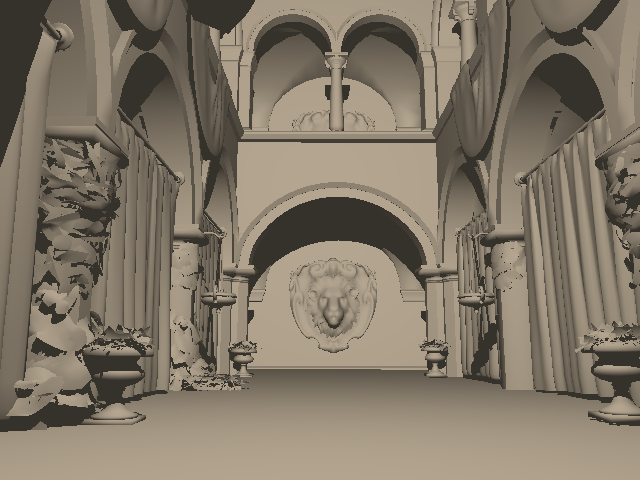
\includegraphics[width=12cm]{sponzaInShadow}};
                \draw (2,1.5) node {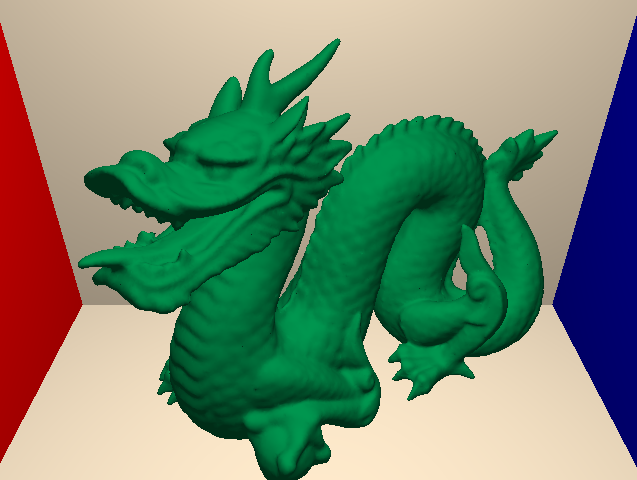
\includegraphics[width=4cm]{opaqueDragon}};
                \draw (6,1.5) node {\reflectbox{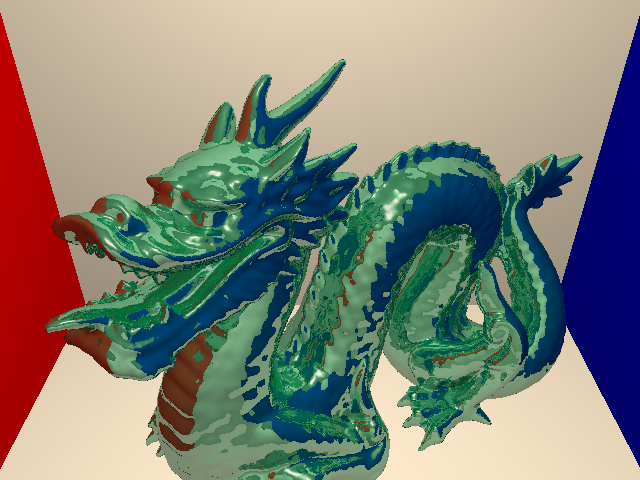
\includegraphics[width=4cm]{semiReflectingDragon}}};
                \draw (10,1.5) node {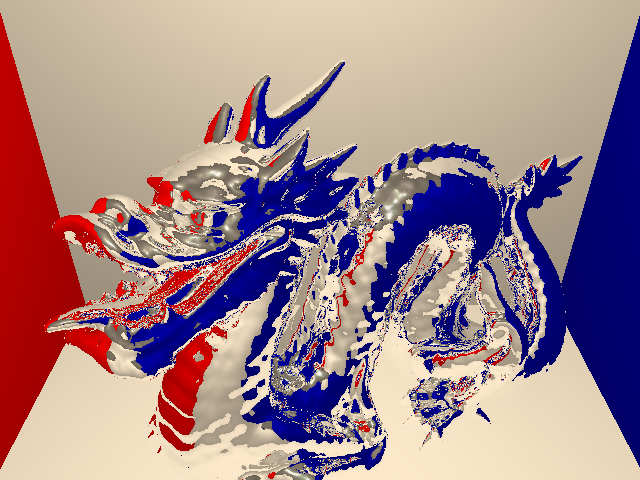
\includegraphics[width=4cm]{reflectingDragon}};
              \end{tikzpicture}
              \vspace*{40pt}
              \\
              \begin{minipage}{0.4\textwidth}
                \centering
                Asger Dam Hoedt \\ asgerhoedt@gmail.com \\ 20051770
              \end{minipage}
              \begin{minipage}{0.4\textwidth}
                \centering
                Thomas Sangild Sørensen \\ sangild@cs.au.dk
              \end{minipage}
    }
    \vfill
    \small
    Department of Computer Science\\
    Aarhus Universitet
\end{titlepage}

\clearpage\pagenumbering{Roman}

%% Isbrief:200-300words. 
%% • Summarizes your work:
%% – What problem does this paper solve?
%% – Why is this problem important for medical image computing (the context and motivation)? 
%% – How does your method work? 
%% – How does it differ from previous work? 
%% – How much better than previous work is it?
%% • There are usually no references in the abstract
%% • The abstract should be readable and understandable by non-experts


\begin{center}
\begin{minipage}{0.7\textwidth}
\section*{Abstract}

This thesis concerns itself with raytracing and doing that efficiently
while exploiting the massive power of todays modern graphics cards. It
is motivated by the ever increasing interest in raytracing and global
illumination for creating effects in movies, but also the increased
usage of 2D and 3D ray tracing used in modern computer games.

The thesis present a survey of different techniques for creating
hierarchical ray tracing acceleration structures, specifically the
binary kd-trees, and how to do this efficiently on the wide SIMT
hardware. A ray tracer will be used to test the quality of the
differently created kd-trees.

While previous work in the area has focused on creating optimal
acceleration structures, the goal of this thesis is to explorer if
spending less time on optimizing the acceleration structures for ray
tracing, can result in an overall performance increase in a dynamic
scene.

To give a fair comparison of the time spend ray tracing and time spend
creating the tree, both generel and SIMT specific optimizations have
been applied to the ray tracer and kd-tree.

\end{minipage}
\end{center}

% Show that to achive raytracing of dynamic scenes, focus should not
% be on creating 'optimal' trees, but instead on creating good trees
% fast.






% Efficiently create KD trees on the GPU and ray trace them.

% KDtree focus will be on optimizations and the tradeoff between
% spending extra time on the kd-tree instead of ray tracing.




\tableofcontents

\clearpage\pagenumbering{arabic}


%\maketitle

%% • The introduction must be dynamite. 
%% – The reader forms an oppinion of the work right from the start... 
%% • The introduction is an extension of the abstract. 
%% • Should be easy to read and understand 
%% • Should make it easy for anyone to tell
%% – What your paper is about 
%%   – What problem it solves
%%   – Why the problem and solution is interesting and relevant (motivation and context). Is it a long- outstanding problem?
%%   – What is new in your paper and how (much) does it improve on the strongest alternatives/previous work (include a few of the most relevant references here).

%% • Start the introduction with the motivation. Think in large contexts and don’t be afraid to be a poet.
%% • All implications, contributions and keypoints of your work must be included here.
%% • Make it very clear how your work will impact the future of Realistic image generation (will people use it?).
%% • If your work is pioneering, s-p-e-l-l i-t o-u-t.
%% • Briefly make it clear how you evaluate your method in the Results section.
%% • Make sure to explain where your method applies and where it does not apply (limitations).


\chapter{Introduction}

\chapterquote{Focus is a matter of deciding what things you're not
  going to do.}{John Carmack}


% Motivation

\textit{Rendering} is the process of converting a scene description into an
image and lies at the heart of \textit{computer graphics}. The ability to render
complex scenes realistically or distinctly is vital in several areas; computer
games, movies and even medical imaging. A scene is made up of models, which can
consist of several thousand geometric primitives, usually triangles. 
%\fixme{Kan dette gøres mere læsevenligt?}
Information about these triangles are stored at the vertices and can be its
position, a normal perpendicular to its surface or its color among other
things. Such information stored at triangle vertices are called \textit{vertex
  attributes}.


% Rasterization and cube mapping

When real-time rendering is needed, the technique of choice for the last one and
a half decade has been \textit{rasterization}. In rasterization a geometric
primitive's vertex attributes are mapped onto a \textit{raster}\footnote{A flat,
  2D grid.} and used to calculate the color of individual raster cells. This
technique is so popular in the gaming industry that processing units were
created specifically for rasterization, the \textit{Graphics Processing Unit} or
\textit{GPU} for short. Due to the industry's ever increasing demand for more
detailed models and visual effects, the GPUs have seen a massive increase in
both computational power and memory bandwidth over the last
decade. Unfortunately, even with all this power, certain aspects of rendering are
still not easily solved by rasterization. \textit{Reflection} and
\textit{refraction} effects on non-flat surfaces are still notoriously hard to
recreate. The reason is that the reflection of complex objects can not easily be
mapped to a two dimensional grid, such as the raster. Reflections of complex
objects can be approximated by \textit{environment mapping} or \textit{cube
  mapping}, of which a short describtion can be found on \reffig{fig:cubemap}. A
problem with cube mapping is that the scene must to be rendered once for each
side of the cube map, which increases the cost of rendering a scene
drastically. Another shortcoming of cube mapping is that it does not support
\textit{self reflection}, since it is only the surrounding environment that is
rendered onto the map.

\begin{figure}
  \centering
  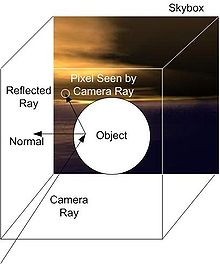
\includegraphics{Cube_mapped_reflection_example}

  \vspace{3mm}
  \parbox{9.5cm}{\caption[Cube mapping visualized.]{A visualization of cube
      mapping. The environment is rendered onto the sides of the cube and then
      mapped onto the object inside the cube map. The mapping is performed by
      using the calculated reflection vector as an index into the cube
      map.\\Image from
      http://en.wikipedia.org/wiki/Reflection\_mapping}\label{fig:cubemap}}
\end{figure}

% Ray tracing and comparing it to rasterization

An alternative to rasterization is \textit{ray tracing}, which elegantly solves
reflection and refraction by tracing rays from the viewer's eye and into the
scene, spawning and tracing new reflection- and refraction rays as needed when
geometry is intersected. 
A comparisson of cube mapping and ray tracing can be seen on
\reffig{fig:reflectingDragons}. The reflecting Stanford Dragon on
\reffig{fig:reflectingDragons} has been rendered by me, as have all images in
this thesis unless explicitly stated
%% A comparisson of cube mapping and ray tracing is given in
%% \reffig{fig:reflectingDragons}, where I have rendered a reflecting Stanford
%% Dragon using both techniques.
Notice how the ray traced dragons backside reflects its neck, while the cube
mapped version only reflects the surrounding box. Advanced lighting techniques
that produce photorealistic images are also based on ray tracing. One such
technique is \textit{photon mapping}, which can accurately reproduce the effects
of light bouncing of reflective surfaces, caustics and color bleeding.

\begin{figure}
  \centering
  \subfloat[A cube mapped reflecting dragon.]{
    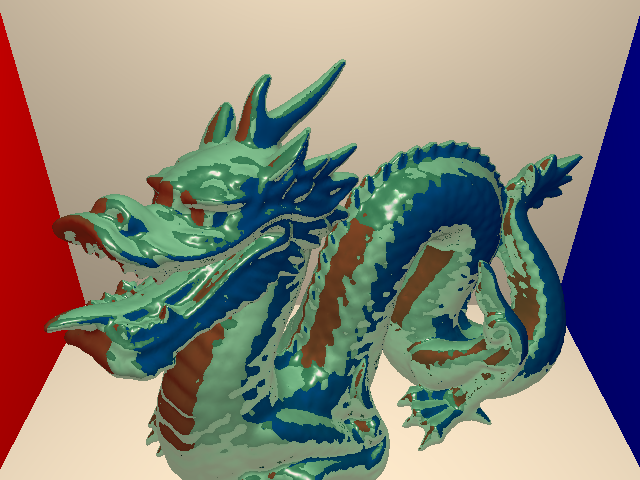
\includegraphics[width=7cm]{cubemappedDragon}
    \label{fig:cubeDragon}
  }
  \hspace{10pt}
  \subfloat[A ray traced reflecting dragon. Notice the self reflection
    on the back and inside the mouth.]{
    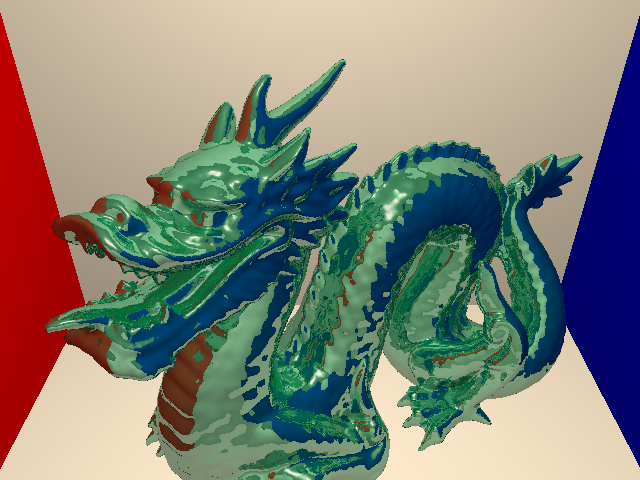
\includegraphics[width=7cm]{semiReflectingDragon}
    \label{fig:rayReflectingDragon}
  }
  \caption[Reflections created with cube mapping and ray tracing.]{An example of
    the difference between using cube mapping or ray tracing for
    reflections.}
  \label{fig:reflectingDragons}
\end{figure}


% High cost used to make it unattractive for interactive scenes.  What I will
% show, doing it dynamically, which is interesting for games and movie
% development

The increased realism that can be achieved by using ray tracing does come at a
high computational cost, which has previously made it unattractive for
interactive applications or dynamic scenes. Nonetheless, the continued increase
in computational power of both CPUs and GPUs, coupled with research into the
area of \textit{interactive ray tracing}, has yielded some remarkable results.
Scenes of approximately 100k triangles can now be ray traced in real-time, even
with effects such as shadows, reflection and refraction added. This makes ray
tracing an increasingly more interesting alternative to rasterization. In this
thesis I will examine \textit{ray tracing of dynamic scenes}, with the express
goal to minimize the time between modifying the scene and presenting a viewer
with visual feedback of the change. This would be very interesting in the film
industry, where ray tracers are used to create
\textit{CGI}\footnote{Computer-generated Imagery} effects and 3D artists need
fast visual feedback while modifying the scene.

%% In this thesis I will examine \textit{ray tracing of dynamic scenes}, which is
%% becoming an interesting alternative to rasterization in the gaming industry in
%% the years to come. The film industry has also used ray tracing to do their
%% \textit{CGI}\footnote{Computer-generated Imagery} effects for quite some time,
%% and for the 3D artists working on these effects, it would certainly be
%% beneficial to use a ray tracer that is able to produce fast visual feedback,
%% when an artist rearranges the scene.

% We need Acceleration stuctures for ray tracing to achieve this

To improve the performance of ray tracers, several acceleration structures have
been developed. The most popular structures are \textit{hierarchical data
  structures}, such as trees, and ray tracers that traverse these are called
\textit{hierarchical ray tracers}. When a ray traverses a hierarchical data
structure it is in search of the nearest leaf node, which contains references to
the geometry nearest to the ray. If the ray finds that it did not see, or
\textit{intersect}, any of the geometry in the current leaf node, it advances
beyond that leaf and performs another traversal of the structure.

The structure employed in this thesis is the \textit{kd-tree}, a binary, space
partitioning tree-structure, which recursively subdivides $k$-dimensional
geometry by splitting it with an \textit{axis aligned splitting plane}. Each
interior node in the tree contains a splitting plane and a reference to the
location of its left and right children, while the leafs contain references to
the geometry associated with them.
%% An example of a subdivided scene and the corrosponding tree can be seen on
%% \reffig{fig:kdIteration} in \refchapter{chp:kdTrees}, where kd-trees will be
%% introduced thoroughly. 
If a leaf node is split by a splitting plane, the geometry associated with that
leaf must be associated with its two newly constructed child nodes. The quality
of a kd-tree is defined as the ease with which it allows a scene to be ray
traced and is affected by the choice of splitting planes. A lot of computational
power can go into finding optimal splitting planes, as there are infinitely many
possible \textit{splitting plane candidates}, or \textit{split candidates}, to
consider.

%% In a high quality kd-tree, splitting planes have been chosen such that
%% spatially close geometry are allocated into the same subtree and the scene
%% can be ray traced as fast as possible. Choosing a splitting plane for a node
%% is the topic of \refsection{sec:splittingPlane}.

In order to facilitate dynamic scenes, the data structure must also be
dynamic. It is possible to dynamically add and remove elements to a kd-tree, but
doing so can degrade the quality of the kd-tree or its subtrees. If a subtree's
quality has degraded too much, it will have to be restructured to facilitate
fast ray tracing again. In the worst case scenario this restructuring needs to
be performed on the entire tree and is equivelant to a complete
reconstruction. Because of this, the algorithms for creating and restructuring
kd-trees needs to be very fast, and might even have to sacrifice tree quality
for improved construction speed. This tradeoff between speed and quality is also
what makes dynamic scenes interesting compared to static scenes. Ray tracers
rendering static scenes can use as much time as needed to produce acceleration
structures of high quality. This may not be possible in dynamic scenes, where a
user modifying the scene will want visual feedback of the modifications made
as fast as possible.

In general there are three ways to optimize ray tracing with respect to dynamic
scenes to achieve maximum efficiency:

\begin{enumerate}
  \item \textbf{Building a higher quality acceleration structure -} An
    acceleration structure of higher quality will reduce the time it takes the
    ray tracer to find the nearest intersecting point between a ray and the
    scene. Algorithms for producing kd-tree's of different quality is the topic
    of \refsection{sec:buildingTrees}.
  \item \textbf{Build the acceleration structure faster -} As described above,
    the acceleration structure may need to be entirely reconstructed each time a
    dynamic scene is rendered. Being able to rebuild it fast is therefore
    crucial. One way to ensure a faster reconstruction is by reducing the time
    spent deciding where to place the splitting plane, which can result in trees
    of lower quality.
  \item \textbf{Create a faster ray tracer -} Several optimizations exist that
    improve the speed of a ray tracer without modifying the underlying
    acceleration stucture. Such optimizations will be discussed in
    \refsection{sec:hierarchicalTraversal}.
\end{enumerate}


% Why do it on the GPU, yes why indeed? Leaves the CPU free to do
% other things than rendering.

As observed at the beginning of this chapter, GPUs have grown quite powerful
over the last decade, and since the introduction of programmable GPUs and
NVIDIA's \textit{CUDA}\footnote{Compute Unified Device Architecture.}
framework, many algorithms have been succesfully ported to utilize the resources
of the GPU. In this thesis I too will use the massive computational power of the
GPUs to accelerate the creation of data structures and ray tracing them. The
most compelling reason to do this, is that it leaves the CPU free to handle
other aspects of a graphics application, such as user input and network
communication.

%% However, the results achieved in this thesis with respect to ray tracing dynamic
%% scenes are architecture independent and apply to the CPU aswell as the GPU.

%% Describe and reference previous work that is relevant to your work.

%% The previous work section is mostly descriptive.

%% Address the weaknesses of the previous methods.

%% You should not do a full comparison between your method and previous
%% work here. Leave that for the Results section.

%% You can however distinguish yourself from previous work by saying
%% something like ”In contrast to method X, my method...”, or ”The main
%% difference between my work and X is...”.

\newpage
\fixme{Make sure this starts on a newline if needed}

\section{Previous Work}

\chapterquote{If you want to make an apple pie from scratch, you must
  first create the universe.}{Carl Sagan}


% Early ray tracing

Arthur Appel\citebook{Appel:1968} is credited as the being the first to describe
the basic idea of ray casting, applying it to solve the \textit{hidden surface
  problem} and to enhance the perception of depth by computing shadows in opaque
polygonal scenes. Whitted\citebook{Whitted:1979} extended the idea of ray
casting into the general recursive ray tracing algorithm still used today. If a
ray would hit a surface, then depending on the surface's material proporties it
could generate any number of new rays, reflection, refraction or shadow.


% Data structures for acceleration

Since then a lot of time and effort has gone into improving the performance of
ray tracing and several data structures have been proposed with this in mind. In
1976 Clark\citebook{Clark:1976:HGM:360349.360354} was the first to suggest using
\textit{bounding volumes} to perform geometry culling and in 1986 Goldsmith and
Salmon\citebook{Goldsmith:1987} extended this idea with an algorithm for
automatically building \textit{bounding volume hierarchies}, \textit{BVH}'s,
topdown. Fujimoto, Tanaka and Iwata\citebook{Fujimoto:1986} introduced the use
of \textit{uniform voxel grids} in 1986. Kaplan\citebook{Kaplan:1985} introduced
the use of kd-trees as a spatial partitioning scheme. To decide where to place
the splitting plane he used the now standard \textit{spatial median splitting}
algorithm. Spatial median splitting places the splitting plane at the middle of
a node's bounding box along some axis, usually either the longest or an axis
chosen in a \textit{round robin} fassion.


% Surface Area Heuristic 

The idea of automatically creating hierarchical acceleration structures have
since been revisited and improved upon countless times. One of the most
important improvements was the introduction of the \textit{Surface Area
  Heuristic}, \textit{SAH}, generally attributed to MacDonald and
Booth\citebook{MacDonald:1990}. SAH estimates the expected cost of ray tracing a
node's two child nodes with respect to some splitting plane. Given a list of
splitting planes, the expected cost for all these planes can then be calculated
and the plane with least cost is chosen as the splitting plane.
%% How exactly this list of splitting planes is created in the first place will be
%% discussed in \refsection{sec:splittingPlane}.


% Havran and kd trees are best?

In his ph.d. thesis\citebook{Havran:PhD} from 2000, Havran argued that the
kd-tree was the best known acceleration structure for ray tracing. While a lot
of new data structures have since appeared, the kd-tree is still one of the most
widely used structures due to its low memory footprint, fast ray/plane
intersection test and countless research papers devoted to both optimal creation
and ray tracing. For these same reasons this thesis will focus on the use of
kd-trees as its acceleration structure.



% GPU acceleration structures

Because of the lack of looping and branching on early programmable graphics
hardware, the first all GPU based ray tracers had to make use of non
hierarchical acceleration structures like grids\citebook{844181}. Grid's,
however, do not scale aswell as hierarchical structures and, in large sparse
scenes, fine-grained grids run the risk of wasting memory on a lot of empty
cells, while more coursely grained grids might store most of the geometry in a
few cells and thus not partition it effectively.

% Traversing the tree and doing it fast

With the addition of branching and looping on graphics hardware, several GPU
based hierarchical ray tracers were proposed. A known optimization to CPU based
hierarchical ray tracers is to use a stack of neighbouring nodes that the ray
could possibly traverse. This is used as a means to prevent restarting ray
tracing from the root of the acceleration structure, if a ray does not intersect
any primitives in its current leaf. Small amounts of available memory per thread
on the graphics card made this optimization technique infeasable for GPU
solutions. Instead Popov et al.\citebook{popov:07:GPURT} in 2007 introduced a
stackless ray tracer rivalling CPU ray tracers in speed, which preprocessed the
kd-tree and adds \textit{ropes}, or references, between neighbouring
nodes. Concurrently \horn{} proposed a different but equally effective
solution. Instead of storing the entire stack of possible neighbouring nodes, a
\textit{short-stack} of only the $N$ lowest possible nodes was stored in
memory. Horn et al. also introduced an optimization called \textit{push-down},
where each ray did not restart at the root of the tree, but instead at the root
of the smallest subtree enclosing the ray. Finally they showed how this could be
implemented together with \textit{packet tracing}, where several rays are traced
in packets by one thread to amortize the cost of traversing the tree.

%% In this thesis I've adopted Horn et al.'s idea of a short stack to
%% improve our ray tracer. In a worst case scenario where all the rays
%% are intersecting the root node's splitting plane, the push-down approch
%% yields no improvement, but only adds a computational overhead, which
%% can also be seen in the papers results section. Therefore I have
%% chosen not to implement it. With the increased detail in ray traced
%% scenes, ray directions may become more and more chaotic after the
%% primary rays have been cast. Due to this, packet tracing may not be
%% one of the best long term optimizations. In this thesis I will instead
%% show how grouping spatially close primary rays into clusters will
%% drastically improve ray tracing efficiency, with hardly any added
%% extra logic.


% Previously constructing the KD-tree was most effective on the CPU,
% optimized and fast for multi core CPU's

Although ray tracing on graphics hardware had been made as fast as its CPU
counterparts by 2007, creating kd-trees on the GPU had still not been done
efficiently.

% Recent research has made it possible to construct KD-trees
% efficiently on GPU's

This changed in 2008 when \zhou{} introduced \textit{breath-first} tree creation
on the GPU. Instead of creating kd-trees in \textit{depth-first} manner, in
which only one node was processed at a time, their breath-first algorithm made
it possible to work on hundreds or thousands of nodes in parallel, allowing it
to scale much better with the architecture of graphics cards. For the uppermost
nodes in the tree they proposed to parallelize the calculation of the node split
cost across all geometric primitives, creating thousands of threads. For the
lower part of the tree, where thousands of nodes needed to calculate their split
cost, computations were simply parallelized over all available nodes.


% KD-tree work and what we've made differently

%% The kd-tree construction work done in this thesis is greatly inspired
%% by Zhou et al.\citebook{1409079}. My approch to upper tree nodes is
%% nearly identical to theirs; using spatial median splitting for
%% determining where to place the splitting plane and optimizing the tree
%% by maximizing empty space. I will however also be focusing on how to
%% handle triangles cut by the splitting plane and discuss 2 alternatives
%% to a standard splitting approach. In the case of lower nodes I will
%% compare the computation intensive SAH, as used by \zhou, to 2 other
%% methods. The first trivially stops tree creation at the upper trees
%% leafs, while the second method will create balanced subtrees.


\section{Goals}

In this thesis the goal is not to produce images of photorealistic quality, or
create an interactive ray tracer \footnote{This goal alone can be achieved
  trivially by reducing the complexity of the ray traced scene or lowering the
  image resolution.}. Instead this thesis will explorer ray tracing acceleration
structures, specifically the kd-tree, and its impact on ray tracing efficiency
for dynamic scenes.

The main topic in this thesis is the relationship between the time spend
constructing a kd-tree and its resulting quality, i.e. how fast can it
accelerate ray tracing. Building on the kd-tree implementation presented by
\zhou{}, I will investigate different parts of the kd-tree construction phase
for dynamic scenes and whether it is worthwile in dynamic scenes to sacrifice
tree quality in order to gain faster kd-tree construction. The two parts of the
kd-tree creation phase that will be investigated is the choice of splitting
plane and how geometry is associated with child nodes after a split. As part of
this investigation I will describe several different solutions and show how to
implement them efficiently on dataparallel GPUs using CUDA.

The kd-trees created by the different methods above will be evaluated by how
fast they can be constructed and how efficiently a ray tracer can traverse them
to render a scene. During evaluation I will always perform a complete rebuild of
the kd-tree before rendering a scene. This is done to ensure that my tests
capture the worst case scenario for dynamic scenes, which is a complete update
of the entire scene and thus a complete rebuild. The goal of this thesis is then
to find a kd-tree configuration that minimizes the total time spent both
recreating and traversing the acceleration structure and evaluate the tradeoff
between construction speed and tree quality.

I will furthermore discuss the ray tracers used to evaluate the quality of the
kd-trees. To provide a fair and useful comparison of a kd-tree's construction
time and its quality, I will need to create a highly optimized ray tracer. These
optimizations are important as a fully optimized ray tracer can render scenes up
to 70\% faster than a basic implementation and does so independent of the
underlying kd-tree and its construction schemes. While I will be discussing and
applying these optimizations, such as the short-stack optimization from \horn{},
the topic is secondary to kd-trees and merely included for evaluation purposes.

Given the added overhead of continuously rebuilding the kd-trees, an interesting
question is whether or not we even need them. I therefore present an
\textit{exhaustive ray tracer}, which does not use any acceleration structure
and thus intersects every ray with every triangle. The exhaustive ray tracer
will be compared to the hierarchical ray tracers and hopefully motivate the
continued use of acceleration structures for dynamic scenes.

\section{Overview}

The rest of the thesis is structured as follows:

% Understanding CUDA

\Refchapter{chp:GPGPU} introduces NVIDIA's CUDA framework. Here I will describe
its thread and memory model. I will then go on to describe a new primitive
proposed by \sengupta{}, which will be needed during kd-tree construction,
e.g. when assigning triangles to child nodes after their parent node has been
split. The last part of this chapter will focus on optimization techniques
specific to CUDA and apply these incrementally in a case study of a global
minima algorithm.

% kd-trees

\Refchapter{chp:kdTrees} is devoted to discussing the construction of
kd-trees. The first part of this section deals with the general kd-tree
construction algorithm. Here I will present several algorithms for choosing the
splitting plane and discuss three different approaches used to associate
triangles with leaf nodes. The second part of \refchapter{chp:kdTrees} deals
with the actual implementation of kd-trees on a GPU and will describe how the
nodes are structured in memory and how to construct binary trees effectively on
dataparallel hardware.

% ray tracing

Having introduced kd-trees, \refchapter{chp:rayTracing} will deal with the
algorithms for traversing such trees and ray tracing a scene. Here several
optimizations to a basic hierarchical ray tracer will be discussed and
incrementally added. First though, an exhaustive ray tracer is presented and
will be used in the Conclussion to motivate the use of hierarchical data
structures. This chapter also includes a discussion of two triangle intersection
algorithms with respect to achieving maximal performance on GPUs.

% Results

In \refchapter{chp:results} I will first evaluate the performance of several
different ray tracers. I will then use the ray tracer that generally performs
best to evaluate the quality of the different kd-trees created. The metric used
to determine which kd-tree construction algorithm performs best will be the
total rendering time, i.e. the sum of the construction time and ray tracing
time.

% Conclusion % Future work

I will then conclude my work by discussing my results and their implications for
the future of ray tracing dynamic scenes. Finally in \refchapter{chp:future} I
will address future improvements based on the experience I have gained while
working on this thesis.



%% Describe and reference previous work that is relevant to your work.

%% The previous work section is mostly descriptive.

%% Address the weaknesses of the previous methods.

%% You should not do a full comparison between your method and previous
%% work here. Leave that for the Results section.

%% You can however distinguish yourself from previous work by saying
%% something like ”In contrast to method X, my method...”, or ”The main
%% difference between my work and X is...”.

\newpage
\fixme{Make sure this starts on a newline if needed}

\section{Previous Work}

\chapterquote{If you want to make an apple pie from scratch, you must
  first create the universe.}{Carl Sagan}


% Early ray tracing

Arthur Appel\citebook{Appel:1968} is credited as the being the first to describe
the basic idea of ray casting, applying it to solve the \textit{hidden surface
  problem} and to enhance the perception of depth by computing shadows in opaque
polygonal scenes. Whitted\citebook{Whitted:1979} extended the idea of ray
casting into the general recursive ray tracing algorithm still used today. If a
ray would hit a surface, then depending on the surface's material proporties it
could generate any number of new rays, reflection, refraction or shadow.


% Data structures for acceleration

Since then a lot of time and effort has gone into improving the performance of
ray tracing and several data structures have been proposed with this in mind. In
1976 Clark\citebook{Clark:1976:HGM:360349.360354} was the first to suggest using
\textit{bounding volumes} to perform geometry culling and in 1986 Goldsmith and
Salmon\citebook{Goldsmith:1987} extended this idea with an algorithm for
automatically building \textit{bounding volume hierarchies}, \textit{BVH}'s,
topdown. Fujimoto, Tanaka and Iwata\citebook{Fujimoto:1986} introduced the use
of \textit{uniform voxel grids} in 1986. Kaplan\citebook{Kaplan:1985} introduced
the use of kd-trees as a spatial partitioning scheme. To decide where to place
the splitting plane he used the now standard \textit{spatial median splitting}
algorithm. Spatial median splitting places the splitting plane at the middle of
a node's bounding box along some axis, usually either the longest or an axis
chosen in a \textit{round robin} fassion.


% Surface Area Heuristic 

The idea of automatically creating hierarchical acceleration structures have
since been revisited and improved upon countless times. One of the most
important improvements was the introduction of the \textit{Surface Area
  Heuristic}, \textit{SAH}, generally attributed to MacDonald and
Booth\citebook{MacDonald:1990}. SAH estimates the expected cost of ray tracing a
node's two child nodes with respect to some splitting plane. Given a list of
splitting planes, the expected cost for all these planes can then be calculated
and the plane with least cost is chosen as the splitting plane.
%% How exactly this list of splitting planes is created in the first place will be
%% discussed in \refsection{sec:splittingPlane}.


% Havran and kd trees are best?

In his ph.d. thesis\citebook{Havran:PhD} from 2000, Havran argued that the
kd-tree was the best known acceleration structure for ray tracing. While a lot
of new data structures have since appeared, the kd-tree is still one of the most
widely used structures due to its low memory footprint, fast ray/plane
intersection test and countless research papers devoted to both optimal creation
and ray tracing. For these same reasons this thesis will focus on the use of
kd-trees as its acceleration structure.



% GPU acceleration structures

Because of the lack of looping and branching on early programmable graphics
hardware, the first all GPU based ray tracers had to make use of non
hierarchical acceleration structures like grids\citebook{844181}. Grid's,
however, do not scale aswell as hierarchical structures and, in large sparse
scenes, fine-grained grids run the risk of wasting memory on a lot of empty
cells, while more coursely grained grids might store most of the geometry in a
few cells and thus not partition it effectively.

% Traversing the tree and doing it fast

With the addition of branching and looping on graphics hardware, several GPU
based hierarchical ray tracers were proposed. A known optimization to CPU based
hierarchical ray tracers is to use a stack of neighbouring nodes that the ray
could possibly traverse. This is used as a means to prevent restarting ray
tracing from the root of the acceleration structure, if a ray does not intersect
any primitives in its current leaf. Small amounts of available memory per thread
on the graphics card made this optimization technique infeasable for GPU
solutions. Instead Popov et al.\citebook{popov:07:GPURT} in 2007 introduced a
stackless ray tracer rivalling CPU ray tracers in speed, which preprocessed the
kd-tree and adds \textit{ropes}, or references, between neighbouring
nodes. Concurrently \horn{} proposed a different but equally effective
solution. Instead of storing the entire stack of possible neighbouring nodes, a
\textit{short-stack} of only the $N$ lowest possible nodes was stored in
memory. Horn et al. also introduced an optimization called \textit{push-down},
where each ray did not restart at the root of the tree, but instead at the root
of the smallest subtree enclosing the ray. Finally they showed how this could be
implemented together with \textit{packet tracing}, where several rays are traced
in packets by one thread to amortize the cost of traversing the tree.

%% In this thesis I've adopted Horn et al.'s idea of a short stack to
%% improve our ray tracer. In a worst case scenario where all the rays
%% are intersecting the root node's splitting plane, the push-down approch
%% yields no improvement, but only adds a computational overhead, which
%% can also be seen in the papers results section. Therefore I have
%% chosen not to implement it. With the increased detail in ray traced
%% scenes, ray directions may become more and more chaotic after the
%% primary rays have been cast. Due to this, packet tracing may not be
%% one of the best long term optimizations. In this thesis I will instead
%% show how grouping spatially close primary rays into clusters will
%% drastically improve ray tracing efficiency, with hardly any added
%% extra logic.


% Previously constructing the KD-tree was most effective on the CPU,
% optimized and fast for multi core CPU's

Although ray tracing on graphics hardware had been made as fast as its CPU
counterparts by 2007, creating kd-trees on the GPU had still not been done
efficiently.

% Recent research has made it possible to construct KD-trees
% efficiently on GPU's

This changed in 2008 when \zhou{} introduced \textit{breath-first} tree creation
on the GPU. Instead of creating kd-trees in \textit{depth-first} manner, in
which only one node was processed at a time, their breath-first algorithm made
it possible to work on hundreds or thousands of nodes in parallel, allowing it
to scale much better with the architecture of graphics cards. For the uppermost
nodes in the tree they proposed to parallelize the calculation of the node split
cost across all geometric primitives, creating thousands of threads. For the
lower part of the tree, where thousands of nodes needed to calculate their split
cost, computations were simply parallelized over all available nodes.


% KD-tree work and what we've made differently

%% The kd-tree construction work done in this thesis is greatly inspired
%% by Zhou et al.\citebook{1409079}. My approch to upper tree nodes is
%% nearly identical to theirs; using spatial median splitting for
%% determining where to place the splitting plane and optimizing the tree
%% by maximizing empty space. I will however also be focusing on how to
%% handle triangles cut by the splitting plane and discuss 2 alternatives
%% to a standard splitting approach. In the case of lower nodes I will
%% compare the computation intensive SAH, as used by \zhou, to 2 other
%% methods. The first trivially stops tree creation at the upper trees
%% leafs, while the second method will create balanced subtrees.


\chapter{Understanding the GPGPU}\label{chp:GPGPU}

\chapterquote{Hardware: The parts of a computer system that can be
  kicked.}{Jeff Pesis}



% Motivate the use of GPUs

Because of the evergrowing demand for new effects and more detail in
computer games and other 3D graphics applications, GPU's have seen a
massive increase in power over the last decade, as evidenced by
\reffig{fig:gflops}. A similar figure comparing the theoretical
throughput of GPU's and CPU's can be seen in \citebook{CUDAPG}. With
this in mind it is easy to understand why one would want to perform
ray tracing entirely on the GPU.

\begin{figure}
  \centering
  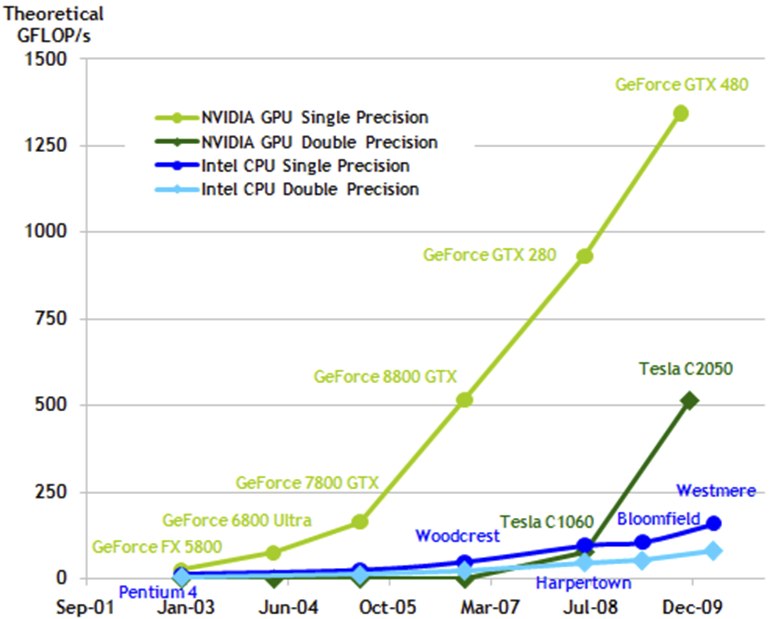
\includegraphics[width=8cm]{GFLOPS}
  \caption{A comparison of the development of floating point
    operations per second on GPU's and CPU's. \\The figure is borrowed
    from Chapter 1 in \citebook{CUDAPG}.}
  \label{fig:gflops}
\end{figure}

% What is different form CPUs

Utilizing all this power effectively, however, is not straightforward
and in order to create algorithms on the GPU that run faster than their
CPU counterparts, we need to understand how the GPU works.

The reason behind the difference in theoretical throughput seen in
\reffig{fig:gflops}, is that the CPU is designed for handling all
kinds of problems, with a large cache at it's disposal and efficient
handling of control flow. The GPU on the other hand is designed for
high throughput of small, arithmetically intense, \textit{dataparallel
  programs}\footnote{Each processor performs the same instruction
  concurrently on multiple data elements.} called \textit{kernels},
which is exactly what is required of a graphics card processing
thousands of independent vertices and performing the same shading on
hundreds of thousands of color fragments.

Since the graphics card is designed to perform vertex and fragment
processing independently of their respective neighbouring threads,
this also means that when programming the graphics card, no
assumptions can be made about which thread is where in it's
execution. This presents a problem in cases where the $n$'th thread
depends on information from all previous $n-1$ threads, fx when
splitting data or calculating the minimum or maximum values of $N$
vertices. NVIDIA's CUDA remedies this somewhat by providing
synchronization commands, but since these will only synchronize a
subset of the running threads, the overall problem remains the same.

% Why not use GPU/CPU solutions

An obvious solution is ofcourse to perform easily parallisable
operations on the graphics card and leave the rest for the
CPU. However, the following quote comes to mind:

\quotebook{
  It is important to include the overhead of transferring data to and
  from the device in determining whether operations should be
  performed on the host or on the device.
}{CUDABPG}

So once it has decided to use the graphics card, one cannot simply
transfer data back to the CPU in order to perform some operation and
then transfer it back the GPU. The overhead would in many cases be too
large to see any performance increase at all.

%% Fortunatly Sengupta et al. has come up with a solution to the
%% scattering problem, which will be discussed further in
%% \refsection{sec:GPUprims}.


% Overview of the chapter

Finding effective GPGPU solutions to the above mentioned problems is
the motivation for this chapter, which is structured as follows.
First we shall take a look at the how threads and memory is organized
on the graphics card. Understanding this will be critical in
developing GPGPU efficient solutions. Then a section will present new
GPGPU scan primitives, which will help us to perform data scattering
and reductions on dataparallel hardware. I will then be discussing a
couple interesting optimization techniques on the GPGPU, while
applying them to a reduction case study.



\section{The Architecture of the GPGPU}

To understand the architecture of the GPGPU, we must first understand the
relationship and layout of threads and then the different kinds of
memory available to threads.

\subsection{The Thread Hierarchy}

% Grid, blocks, warps and threads. We will only deal with the one
% dimensional case.

The graphics card is able to handle execution of more than a million
threads sequentially. Simply considering a graphics application
running at a 1440x900 resolution should convince anyone of this. While
above I have argued that all of these threads are executed
independently of each other, NVIDIA's CUDA architecture does place
these threads in a hierarchy, which provides programmers with some
control over thread execution.

% warps

At the lowest level threads are scheduled and executed completely
parallel in small groups called \textit{warps}\footnote{The term
  originates from weaving, the first parallel thread
  technology.\citebook{CUDAPG}}, usually with a warpsize of 32. While
threads in a warp have their own instruction counter and register
state, and therefore logically can branch independently of
neighbouring threads, a warp can only execute one specific instruction
at a time. The following example should help clarify this.

\begin{algorithmic}
  \IF{threadID < 16}
    \ASSIGN{$x$}{$threadID$}
  \ELSE
    \ASSIGN{$x$}{$32 - threadID$}
  \ENDIF
\end{algorithmic}

% It is a wide SIMD/SIMT, Single-Instruction / Multiple-Thread,
% machine. This means branching hurts. Alot!

The first 16 threads in the warp will evaluate to true and thus
perform the assignment $x \leftarrow threadID$, while the next 16
threads will evaluate to false and execute the alternate statement $x
\leftarrow 32 - threadID$. Since the warp can only perform one
distinct instruction at a time, it will have to first execute $x
\leftarrow threadID$, leaving the last 16 threads idle. It next
executes the else branch, meaning the first 16 threads are left
idling. While this example shows how branching can hurt performance,
when all threads in a warp do not take the same execution path,
knowning that all threads in the warp always are synchronized can also
be very beneficial, as will be shown in
\refsection{sec:loopUnrolling}.

% TODO explain any/all/ballot?

% blocks

Warps are then organized into 3 dimensional \textit{blocks}. Blocks
are expected to reside on the same multiprocessor, which provides them
with a limit as to how many threads they can contain. On current GPU's
the limit can be up to 1024 threads per block. Having threads executed
on the same multiprocessor comes with a few benefits. It is possible
to force synchronized execution of entire blocks at specific points in
the kernels. Threads can then cooperate through fast memory local to
the multiprocessor and use it to share data. Threads can lookup their
\textit{thread index} inside a block through the 3 dimensional
\textit{threadIdx} CUDA built-in variable. Being able to lookup a
threads id is important for working with data. In the one dimensional
case the $n$'th thread will usually process the $n$'th data
element. Without the thread index this would not be possible.

% grid

Blocks are themselves arranged into the uppermost part of the thread
hierarchy, a 2 dimensional \textit{grid}. The amount of data being
processed usually defines how large the grid will be. Just like a
thread can access it's index og id, it can also lookup it's block
index inside the grid through the built-in \textit{blockDim}. A 2
dimensional thread hierarchy can be seen on
\reffig{fig:threadLayout}. The kernels in this thesis will usually
process the data as 1D linear array, so a threads global id can be
calculated as $id \leftarrow blockDim.x * blockIdx.x + threadIdx.x$.

\begin{figure}
  \centering
  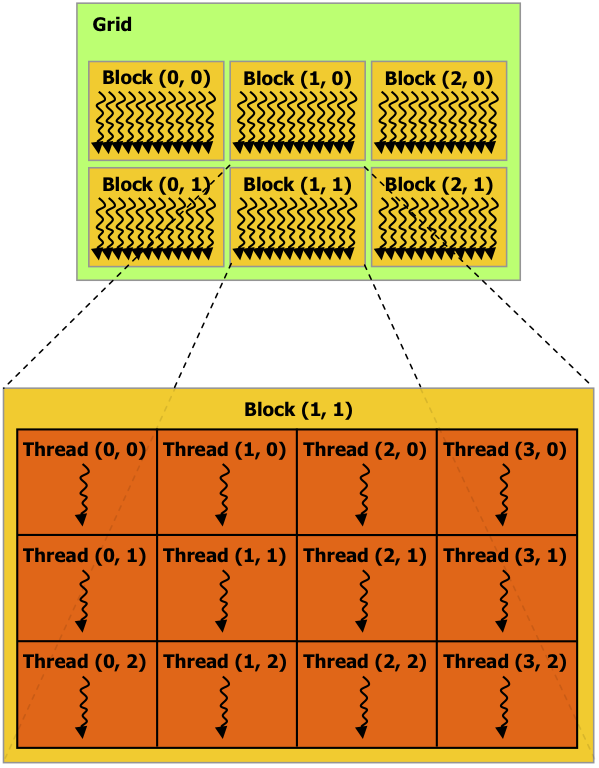
\includegraphics[width=8cm]{ThreadLayout}
  \caption{A figure of CUDA's thread hierarchy.\\ The figure is borrowed
    from Chapter 2 in \citebook{CUDAPG}.}
  \label{fig:threadLayout}
\end{figure}




\subsection{The Memory Model}

With the thread hierarchy explained, the different memory spaces made
available through CUDA can be described.  

CUDA provides the programmer with 3 overall types of memory:
\textit{global memory}, which can be accessed by any thread at any
time and persist across kernel launches, \textit{shared memory}, which
is shared across all threads in a block and persists as long as a
block is active, and finally \textit{registers}, which are local to
each thread and only exists as long as it's thread. In the following
a section is devoted to each memory space.

\subsubsection{Global Memory}

% Slow, coalescene of data types with size 1, 2, 4, 8, and 16 bytes.

Global memory, or \textit{device memory}, is the slowest form of
memory on CUDA devices. As mentioned above it persists across kernel
launches and is therefore perfect for storing input data to kernels
and their results. To avoid making lots of memory transaction to and
from global memory, a warp will try to coalesce it's threads memory
access into as few transactions as possible. How well transactions are
coalesced depends on the \textit{compute capability} of the used
graphics card, with newer graphics cards being more flexible. Suffice
it to say here that it is preferable to access memory sequantially,
ie. the $n$'th thread in a warp accesses the $n$ data element.

% Coalesced memory access, float4 instead of float3
% The alignment requirement can be forced: stuct __align__(8) {

Another restiction on coalescence is that data accessed must be of
size 1, 2, 4, 8 or 16, otherwise memory transactions will be broken up
into multiple requests. Due to this it is actually more efficient to
use the CUDA built-in struct \textit{float4} than \textit{float3}.

Requirements for coalescence on hardware of a specific compute
capability is described in Appendix G of \citebook{CUDAPG}.

% hiding latency

The scheduler can also help with hiding latency from a global memory
access. If one warp is stalled while waiting for data, another
resident warp that is ready to execute can be scheduled
instead. Utilization of the graphics hardware is therefore heavily
dependent on number of resident warps and maximizing this can be
important. Especially if memory accesses are scattered, like they will
be when ray tracing a hierarchical structure.

% Mention textures and cache. The project developed for this thesis
% will not be using textures, since global memory also has cache as of
% 2.0 hardware.

Textures also reside in device memory space. Textures are read only
but provide a fast texture cache, optimized for 2D spatial data
locality. This makes texture access faster than pure global memory
access, as a device memory read is only performed on a cache miss. On
current generation hardware, global memory can use shared memory as a
cache, so textures will not be used in this project.

\subsubsection{Shared Memory}

% Faster than global/local
% Allows threads to share data

Shared memory resides on the multiprocessors and is much faster than
global memory. It is shared by threads across their block, which
allows them to share data.

% Used to overcome the limitations of global memory.

A normal usecase for shared memory is local caching of global data
shared across multiple threads. In this case the kernel first loads
data into shared memory, then performs a block-wide synchronization if
necessary and proceeds to operate on the data in shared memory. When
the kernel has finished it's computations, the data is then dumped
back to global memory.

% Can be used as global cache on never CUDA architectures isntead of
% textures and shared mem. nice we laike

As mentioned above, on newer architecture multiprocessor memory can be
used as a cache for global memory.

% TODO? Bank conflicts, nothing is ever as good as it seems.



\subsubsection{Registers and Local Memory}

% Register

Registers are part of the threads execution context and the fastest
kind of memory on the device. Since there is only a fixed amount of
registers available per multiprocessor, a kernels register usage can
have a high impact on \textit{occupancy}\footnote{The amount of thread
  blocks resident on a multiprocessor, relative to the maximum amount
  possible.}, which in turn can have an impack on the schedulers
ability to hide latency.

% launch bounds

The compiler employs different heuristics to minimize register usage,
while keeping the kernel running efficiently. Sometimes though,
programmers may want to use even fewer registers for specific kernels,
in order to maximize occupancy and global memory latency hiding. To
this end they can aid the compilers heuristics by providing
\textit{launch bounds}. In CUDA 2 arguments can be given as launch
bounds. The first tells the compiler the maximum number of threads per
block that the kernel will ever be invoked with. The second argument
tells the compiler how many blocks should be resident on the
multiprocessor. The compiler can then use this information to derive
upper bounds for the registers per thread.

% TODO? example



% Local memory

But the compiler cannot always simply reduce the number of registers
to fit inside the launch bounds. If 20 register are needed to hold 20
distinct values, then those values have to be stored somewhere else,
if the programmer demands that only 16 registers be used. In that case
the compiler can use \textit{local memory}, which resides in device
memory and thus has the same high latency and low bandwith as global
memory. Forcing a few registers into local memory to gain occupancy
can be beneficial though, and since all threads will access local
memory at the same time, there is a high probability that local memory
access can be coalesced.

Kernel variables that the compiler will most likely place in local
memory are:

\begin{itemize}
  \item Any array that from the compilers point of view are
    dynamically indexed.
  \item Structures or arrays that are to large to fit inside registers.
  \item Any variable in the kernel, if the kernel has to many
    variables to place them all in register memory. This is referered
    to as \textit{register spilling}.
\end{itemize}



\section{The Scan Primitive}\label{sec:GPUprims}

% Motivate

As explained above it can be quite hard to perform reductions and
scattering operations on dataparallel hardware. In this section I will
outline a solution to this problem presented by Sengupta et
al\citebook{Sengupta:2007} and give an example of why this primitive
is important when constructing spatial data structures.

% Prefix sum

The reason for reductions being hard, is that each thread requires
knowledge derived from all threads preceding it. An example taken from
\citebook{Sengupta:2007} is the calculation of a \textit{prefix-sum},
which is a special case of \textit{exclusive scan}. Exclusive scan
takes as input a data array, $[a_0, a_1, a_2, ...]$, and a binary
operator, $\oplus$, with an identity element. The result of exclusive
scan is then a new array with values $[0, a_0, a_0 \oplus a_1, a_0
  \oplus a_1 \oplus a_2, ...]$. For prefix-sum the operator is + and
the identity element is 0.

\begin{displaymath}
  \begin{array}{r r r r r r r r r}
    in: & 3 & 1 & 7 & 0 & 4 & 1 & 6 & 3 \\
    out: & 0 & 3 & 4 & 11 & 11 & 14 & 16 & 22 \\
  \end{array}
\end{displaymath}

Calculating the prefix-sum for $n$ elements on the CPU is trivial and
can naively be done in $O(n)$ time. A naive implementation in the GPU
however would require each thread to sum up every previous value on
it's own, yielding a time complexity of $O(n^2)$. Instead a
dataparallel algorithm has to be devised that allows threads
cooperatively solve the problem and doing that as efficiently as the
CPU, ie in $O(n)$ time.


% Algorithm

Sengupta et al.\citebook{Sengupta:2007}'s work-efficient prefix-sum
requires to passes over the data, one called \textit{reduce} and
another called \textit{down-sweep}. The algorithm is depicted on
\reffig{fig:segScan}. The figure shows scan being applied to an array
containing 8 elements. Cells with the same colors represent threads
belonging to the same block. The arrows show how data is moved, one
arrow entering a cell represents a copy, while 2 arraws entering
represents the application of $\oplus$ to the data. In the reduce
phase \reffig{fig:segScan} shows how each block's threads are first
responsible for cooperating on reducing their own values. The result
of this reduction is then passed as input to a new reduction kernel,
yielding the final reduced value.

\begin{figure}
  \centering
  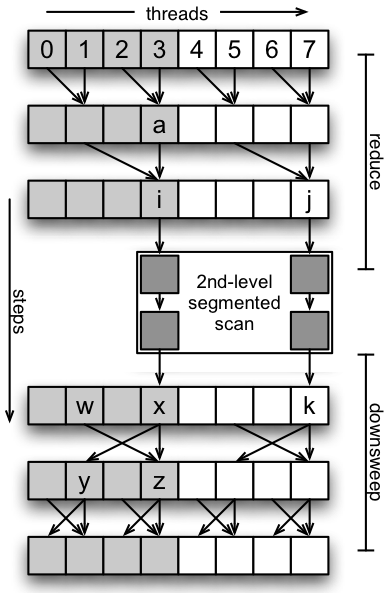
\includegraphics[width=4cm]{SegmentedScan}
  \caption{An example of multi-block segmented scan
    communication. Cells with the same shading belong to the same
    block. \\The figure is borrowed from \citebook{Sengupta:2007}.}
  \label{fig:segScan}
\end{figure}

During down-sweep the data is pumped back out into the array, reusing
the reduced values calculated in the previous phase. The result of
this is an array containing the result of a scan application. It can
be quite instructive in dataparallel programming to go through the
algorithm.

For specific details and further implementation optimizations see
Sengupta et al.\citebook{Sengupta:2007}.


% time complexity

For $n$ elements the time complexity of the parallel scan is $2 * O(n
+ n/2 + n/4 + ... + 1) = O(n)$, since the workload is cut in half for
each iteration of the reduce and down-sweep kernels.


% Useful for splitting data

Now the question is: \textit{why is this useful?}. The answer is that
the prefix-sum is vital to splitting data arrays on the GPU. Imagine
an array of triangles that have been split by a splitting plane and
must now be sorted into a new array, with all triangles in front of
the plane sorted to the left and the triangles behind it sorted to the
left. 

\begin{displaymath}
  \begin{array} {r r r r r r r}
    triangles: & [t_0 & t_1 & t_2 & t_3 & t_4 & t_5]\\
    side: & [r & l & r & l & l & r]\\
  \end{array}
  \Rightarrow
  \begin{array} {r r r r r r r}
    &[t_1 & t_3 & t_4 & t_0 & t_2 & t_5]\\
    &[l & l & l & r & r & r]\\
  \end{array}
\end{displaymath}

This needs to be done every time a tree node is split into 2 child
nodes, so being able to do this efficiently on the GPGPU is imperative
to creating kd-trees efficiently.

Obviously the individual threads in a split kernel will have no idea
where to move the triangle, since that depends on all previous
threads. But by first computing the prefix-sum of the side array,
while adopting the convention that $r = 0$ and $l = 1$, splitting the
triangles become quite easy. Taking the example above the prefix-sum
becomes

\begin{displaymath}
  \begin{array} {r r r r r r r}
    prefix\text{-}sum: & [0 & 0 & 1 & 1 & 2 & 3]
  \end{array}
\end{displaymath}

and the total number of triangles moved left, $nf$, can be found by
adding the last element in prefix-sum with the last element in sides,
which yields $nf = 3 + 0 = 3$.

The observant reader will have noticed that the prefix-sum actually
calculates the addresses where the triangles on the left side should
be moved to. All that remains is then to calculate the addresses of
the triangles moved right. This is done using $right = threadId -
prefix + nf$.

\begin{displaymath}
  \begin{array} {r r r r r r r}
    right: & [4 & 5 & 5 & 6 & 6 & 6]
  \end{array}
\end{displaymath}

The address that a thread should move it's triangle to is then simply
$address = side == l ? prefix : right$ and becomes


\begin{displaymath}
  \begin{array} {r r r r r r r}
    address: & [4 & 0 & 5 & 1 & 2 & 6]
  \end{array}
\end{displaymath}

which will divide the triangles into their respective sides, just like
we wanted.

% TODO? the data keeps it's relation to other elements, which is good
% for coalescence.





% NVIDIA mentioned 3 optimization points

% Structures of arrays vs arrays of structs. Usefull when fx
% sorting. CUDPP article/forum. Plus cache performance.

% Unrolling loops, even when it means more work. Preprocess lower
% nodes yields nearly a 50% speedup from this.


\section{Optimization Techniques: Reduction}\label{sec:reduce}

% Motivation: Reduction was important in the previous step and will be
% again for median splitting

In the previous section we saw that it is important to be able to
perform reductions efficiently on the GPU. Calculating the prefix-sum
however isn't the only part of the kd-tree creator where reductions
are needed. It is also useful for calculating the bounding boxes of
kd-nodes, used when performing median splits.

In this section I will present a naive reduction algorithm and
incrementally apply optimizations to it. The algorithm will use the
binary operator min to find the smallest value from it's input list,
but can be generalized to any reduction. The naive algorithm will have
an efficient time complexity of $O(n)$, which is the best we can hope
for. Instead of improving this time complexity the following
optimizations will instead focus on making better use of the GPU by
hiding latency, using faster memory where available and reduce the
number of calculations made.

% Works on individual blocks, must be run twice if input is too large
% for one block to handle.

The reduction algorithm will reduce values correctly for individual
blocks. If the input list is too large to be efficiently reduced by
one block, then the algorithm can be run recursively on it's own
output, until a single result is found.

The algorithm assumes that the length of the input list is a power of
2. If that is not the case then either the data could be preprocessed
or the kernel itself can pad the data with the binary operators
identity element, in our case $\infty$.

\subsection{Naive implementation}

The naive algorithm, presented in \refalg{alg:naiveReduct}, is a
straight forward implementation of the interleaved access pattern
shown in \reffig{fig:segScan}. The algorithm uses the modulo operator
to distinguish which threads are done and which should continue to
perform reductions. All intermittent values are written back into
global memory, to allow other threads to access the reduced values
when needed. When the block has finished the reduction, the result
is returned by the first thread.

\begin{algorithm}
  \caption{Naive reduction}
  \label{alg:naiveReduct}
  \begin{algorithmic}
    \PROCEDURE{Reduce0}
              {$values$ : Number List; $id$ : Integer; $elements$ : Integer}
              {$result$ : Number}
              {\ASSIGN{$offset$}{$1$}
                \WHILE{$offset < elements$}
                  \IF{$id$ \MOD  $offset = 0$}
                  \ASSIGN{$values[id]$}{\MIN{$values[id]$}{$values[id + offset]$}}
                  \ENDIF
                  \ASSIGN{$offset$}{$offset * 2$}
                  \SYNC
                \ENDWHILE
                \IF{$id = 0$}
                  \ASSIGN{$result$}{$values[0]$}
                \ENDIF
              }
  \end{algorithmic}
\end{algorithm}

\subsection{Coalesced Memory Access}

Ofcourse there are several inefficiencies to correct in
\refalg{alg:naiveReduct}. To start with we will focus on global memory
access and update it to allow the warp to perform memory accesses
coalesced. Since we're interested in a global reduction it won't
matter in which order values are compared. This allows the interleaved
access pattern to be exchanged with a sequential pattern, which will
allow the warp to perform coalesced memory access.

%% Also better warp utilization as most threads are active and we get
%% rid of the slow mod operator.

Two pleasent side effects of this change, as shown in
\refalg{alg:coalescedReduct} is that the slow modulo operator has
disappeared and warp utilization has dramatically increased, since the
first $offset$ threads in a block are now live, compared to every
$offset$'th thread in the previous implementation.

\begin{algorithm}
  \caption{Coalesced reduction}
  \label{alg:coalescedReduct}
  \begin{algorithmic}
    \PROCEDURE{Reduce1}
              {$values$ : Number List; $id$ : Integer; $elements$ : Integer}
              {$result$ : Number}
              {\ASSIGN{$offset$}{$elements / 2$}
                \WHILE{$offset > 1$}
                  \IF{$id < offset$}
                  \ASSIGN{$values[id]$}{\MIN{$values[id]$}{$values[id + offset]$}}
                  \ENDIF
                  \ASSIGN{$offset$}{$offset / 2$}
                  \SYNC
                \ENDWHILE
                \IF{$id = 0$}
                  \ASSIGN{$result$}{$values[0]$}
                \ENDIF
              }
  \end{algorithmic}
\end{algorithm}

% TODO? Figure of sequential access


\subsection{Working from Shared Memory}

Even with coalesced memory acces, continuosly accessing global memory
is still quite slow. To remedy this the implementation in
\refalg{alg:sharedReduct} first copies the data into shared memory
before performing any reductions. As can be seen the threads are
working together to perform the copy. Instead of all threads having to
copy the entire data, each thread only fills the $id$'th cell in the
shared list and leaves the other cells to be filled by the other
threads. The subsequent synchronization ensures that all the data has
been copied before proceding with the reduction. Since the threads are
still accessing data sequentially, this change preserves coalescence.

\begin{algorithm}
  \caption{Shared memory reduction}
  \label{alg:sharedReduct}
  \begin{algorithmic}
    \PROCEDURE{Reduce2}
              {$values$ : Number List; $id$ : Integer; $elements$ : Integer}
              {$result$ : Number}
              {\DECLARE{$sValues$}{\textbf{shared} Number List}
                \ASSIGN{$sValues[id]$}{$values[id]$}
                \SYNC
                \ASSIGN{$offset$}{$elements / 2$}
                \WHILE{$offset > 1$}
                  \IF{$id < offset$}
                  \ASSIGN{$sValues[id]$}{\MIN{$sValues[id]$}{$sValues[id + offset]$}}
                  \ENDIF
                  \ASSIGN{$offset$}{$offset / 2$}
                  \SYNC
                \ENDWHILE
                \IF{$id = 0$}
                  \ASSIGN{$result$}{$sValues[0]$}
                \ENDIF
              }
  \end{algorithmic}
\end{algorithm}

\subsection{Using Registers}

Shared memory is quite fast, but registers are even faster. Inspecting
the statement \MIN{$values[id]$}{$values[id + offset]$}, we can see
that the $id$'th thread will always acces the value stored in
$sValues[id]$ and is the only thread writting to that cell. This
provides us with the possibility to use a register to store this value
in instead. We just have to remember to also store the reduced value
in shared memory, in case another thread needs to use it in the next
iteration. The resulting changes can be seen in
\refalg{alg:registerReduct}.

\begin{algorithm}
  \caption{Register reduction}
  \label{alg:registerReduct}
  \begin{algorithmic}
    \PROCEDURE{Reduce3}
              {$values$ : Number List; $id$ : Integer; $elements$ : Integer}
              {$result$ : Number}
              {\DECLARE{$sValues$}{\textbf{shared} Number List}
                \ASSIGN{$rValue \leftarrow sValues[id]$}{$values[id]$}
                \SYNC
                \ASSIGN{$offset$}{$elements / 2$}
                \WHILE{$offset > 1$}
                  \IF{$id < offset$}
                  \ASSIGN{$rValue \leftarrow sValues[id]$}{\MIN{$rValue$}{$sValues[id + offset]$}}
                  \ENDIF
                  \ASSIGN{$offset$}{$offset / 2$}
                  \SYNC
                \ENDWHILE
                \IF{$id = 0$}
                  \ASSIGN{$result$}{$rValue$}
                \ENDIF
              }
  \end{algorithmic}
\end{algorithm}



\subsection{Loop unrolling}\label{sec:loopUnrolling}

% Unroll the loops: Only works if the number of reductions are known
% beforehand (or if we pad the input)

The final optimization that we will apply to the reduction algorithm
is loop unrolling. As stated above we assume that we know beforehand
how many elements will need to be reduced by the blocks. We now extend
this assumption with the condition that all blocks reduce the same
number of elements. Again this can be accomplished quite easily by
padding the input values when copying them to shared memory. There are
several reason as to why loop unrolling can increase
performance. Firstly looping requires indirection and even though most
of the threads in our warps will loop the same amount of times, the
warps still incur an overhead by having to perform the
indirection. Secondly unrolling removes the overhead of updating the
$offset$ variable, which is a quite significant portion of the work
performed by the kernel when the loop body is as small as
ours. Thirdly we can take advantage of warp synchronization and remove
explicit synchronization invocations when offset becomes less than the
warpsize.

% Then move the first up to where data is loaded into shared mem. And
% move the last reduction down where the final result is written.

After having unrolled the loop, it is now also possible to move thread
0's last reduction, \MIN{$rValue$}{$sValues[1]$}, down to where the
  result is output. We are also able to inline the first reduction
  where the data is copied from global memory to shared memory,
  reducing the shared memory requirements by
  half. \refalg{alg:unrollReduct} shows the inlining of the first and
  final reduction. Unrolling the loop is quite straightforward, but
  takes a lot of space and have therefore been omitted here. 

% Left as an exercise to the reader :)

\begin{algorithm}
  \caption{Unrolling reduction loops}
  \label{alg:unrollReduct}
  \begin{algorithmic}
    \PROCEDURE{Reduce4}
              {$values$ : Number List; $id$ : Integer; $elements$ : Integer}
              {$result$ : Number}
              {\ASSIGN{$offset$}{$elements / 2$}
                \DECLARE{$sValues$}{\textbf{shared} Number List}
                \ASSIGN{$rValue \leftarrow sValues[id]$}{\MIN{$values[id]$}{$values[id + offset]$}}
                \SYNC
                \ASSIGN{$offset$}{$offset / 2$}
                \WHILE{$offset > 2$}
                  \IF{$id < offset$}
                  \ASSIGN{$rValue \leftarrow sValues[id]$}{\MIN{$rValue$}{$sValues[id + offset]$}}
                  \ENDIF
                  \ASSIGN{$offset$}{$offset / 2$}
                  \SYNC
                \ENDWHILE
                \IF{$id = 0$}
                  \ASSIGN{$result$}{\MIN{$rValue$}{$sValues[1]$}}
                \ENDIF
              }
  \end{algorithmic}
\end{algorithm}


\chapter{KD-Trees}\label{chp:kdTrees}

%% \chapterquote{In theory, there is no difference between theory and
%%   practice. But, in practice, there is.}{Jan L. A. van de Snepscheut}

\chapterquote{With todays's fast ray tracers, the difference between a
  ``good'' and a naïvely built kd-tree is often a factor of 2 or
  more.}{Ingo Wald and Vlastimil Havran}



% About KD-trees

Since Arthur Appel described ray tracing four decades ago, several
spatial acceleration structures have been developed to increase the
speed of ray tracers. This chapter will focus on one of the the most
popular acceleration structures, namely the kd-tree.

% Why KD trees

In his ph.d. dissertation \citebook{Havran:PhD}, Vlastimil Havran did
an extensive study of spatial acceleration structures, including
grids, octress and kd-trees. In chapter 3 of the dissertation he
concludes that in most cases the kd-tree will outperform other
well-known acceleration structures.

Since \zhou{}, it has been possible to efficiently construct kd-trees entirely
on the GPU. In the paper they show that their approach even allows ray tracing
dynamic scenes on the GPU, where the kd-tree is reconstructed for each new image
rendered. Building on their approach, I will in \refsection{sec:lowerNodes}
present alternatives to their method for choosing splitting planes. I will also
investigate two different methods for determining when a triangle and a node
overlaps, this is done in \refsection{sec:splittingSchemes}.

Though the different methods and their implementation is presented in this
chapter, the methods will not be evaluated until \refchapter{chp:results}. This
is postponed to allow the introduction of the ray tracers used when evaluating
the quality of the kd-trees in \refchapter{chp:rayTracing}.

% About this Chapter. Start by motivation. Then explain how kd-trees
% are constructed, including different strategies for choosing the
% spliting plane and doing the actual geometry splitting. Then the
% chapter will end with a discussion of how to implement the
% algorithms efficiently on a SIMT architecture.

Before diving into specifics about implementing kd-trees on the GPU, I will
first use the next section to illustrate the recursive kd-tree construction
algorithm in general terms and describe the representation of tree nodes in
memory. The following subsections will then describe different established
algorithms for choosing a splitting plane and how to associate geometry with
child nodes after a split has occured. The latter part of this chapter deals
with converting a single-threaded recursive kd-tree construction algorithm into
a dataparallel algorithm.



\section{Building KD-trees}\label{sec:buildingTrees}

A kd-tree is a binary tree that recursively subdivides k-dimensional geometry
into smaller tree nodes. \Refalg{alg:kdTreeCreator} describes a general
recursive kd-tree construction scheme.

\begin{algorithm}
  \caption{Recursive kd-tree constructor}
  \label{alg:kdTreeCreator}
  \begin{algorithmic}
    \PROCEDURE{CreateNode}
              {$T$ : Triangle List; $voxel$ : AABB}
              {$node$ : Node}
              {\IF{IsLeaf($T, voxel$)}
                  \ASSIGN{$node$}{Leaf(T)}
                \ELSE
                  \COMMENTIT{Determining the splitting plane will be discussed in \refsection{sec:splittingPlane}}
                  \ASSIGN{$plane$}{DeterminePlane($T, voxel$)}
                  \ASSIGN{$(voxel_L, voxel_R)$}{Split($voxel, plane$)}
                  \COMMENTIT{How to associate geometry with a voxel will be the topic of  \refsection{sec:splittingSchemes}}
                  \ASSIGN{$T_L$}{AssociateGeometry($T, voxel_L$)}
                  \ASSIGN{$T_R$}{AssociateGeometry($T, voxel_R$)}
                  \ASSIGN{$node$}{Node($plane$, CreateNode($T_L, voxel_L$), CreateNode($T_R, voxel_R$))}
                \ENDIF}
  \end{algorithmic}
\end{algorithm}


CreateNode takes as arguments a list of triangles and a bounding volume
describing the volume of the node. Usually this bounding volume is an
\textit{axis aligned bounding box}, \textit{AABB}, which is a box whose planes
are aligned with the axes of the coordinate system. An axis aligned bounding
box, $b$, can thus be described by its maximum and minimum values along each
axis and I therefore define it as, $b = \{b_{min}, b_{max}\} \in \{R^3,
R^3\}$. All bounding volumes used in this thesis are axis aligned bounding boxes
and I will therefore use the descriptions bounding volume, bounding box and axis
aligned bounding box interchangeably. CreateNode first checks if the
triangles and the bounding box satisfy the requirements for becoming a leaf
node. If so, then a leaf is produced and the recursion terminates. If not, then
the node's bounding box is divided by a chosen splitting plane, $plane$. How to
determine when to end recursion and choose a splitting plane is the topic of
\refsection{sec:splittingPlane}. Dividing the bounding box produces two new axis
aligned bounding boxes, $voxel_L$ and $voxel_R$. Triangles are then associated
with these new bounding volumes by an association algorithm, which will be
discussed in \refsection{sec:splittingSchemes}. Finally a new node is created
that will contain references to its two children.

An example of an iteration of CreateNode can be seen in
\reffig{fig:kdIteration}. The box surrounding the scene is the bounding volume
of the root node. Before the scene has been subdivided by splitting planes, the
root node itself is a leaf node and therefore contains a list of all triangles
associated with it. In \reffig{fig:simpleScene1} a line has been drawn down the
middle of the scene. This line represents a chosen splitting plane and in the
tree's root node it can be seen that the plane splits along the x-axis at $x=4$,
which corrosponds to what is seen in the scene.

\begin{figure}
  \centering \subfloat[A simple scene and it's corrosponding
    kd-tree. The entire scene is contained in the root node.]{
    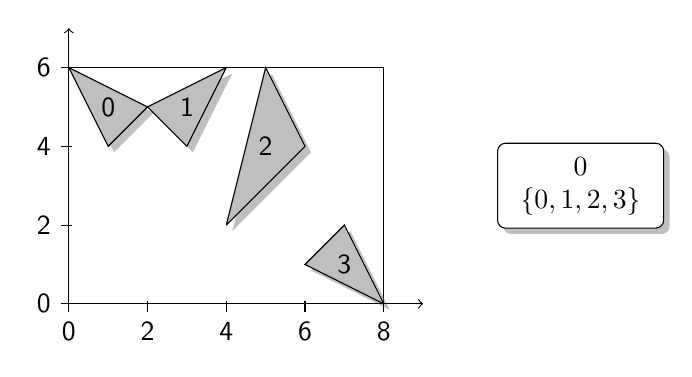
\begin{tikzpicture}[y=0.5cm, x=0.5cm,font=\sffamily]
      \drawNode{0,0}{8,0}{8,6}{0,6}
      
      % Tris
      \drawTri{0,6}{1,4}{2,5}
      \draw (1,5) node{0};
      \drawTri{4,6}{3,4}{2,5}
      \draw (3,5) node{1};
      \drawTri{4,2}{5,6}{6,4}
      \draw (5,4) node{2};
      \drawTri{8,0}{7,2}{6,1}
      \draw (7,1) node{3};

      %axes
      \draw[->] (0,0) -- coordinate (x axis mid) (9,0);
      \draw[->] (0,0) -- coordinate (y axis mid) (0,7);
      %ticks
      \foreach \x in {0,2,...,9}
     		\draw (\x,1pt) -- (\x,-3pt)
			node[anchor=north] {\x};
    	\foreach \y in {0,2,...,7}
     		\draw (1pt,\y) -- (-3pt,\y) 
     			node[anchor=east] {\y}; 

      \draw (13,3) node [leaf] (0){$\begin{array}{c}0\\\{0, 1, 2, 3\}\end{array}$};
    \end{tikzpicture}
    \label{fig:simpleScene0}
  }

  \subfloat[The same scene as in \reffig{fig:simpleScene0}. The kd-tree has
    split the geometry down the middle and created two new leaf nodes, with
    which the geometry has been associated.]{
    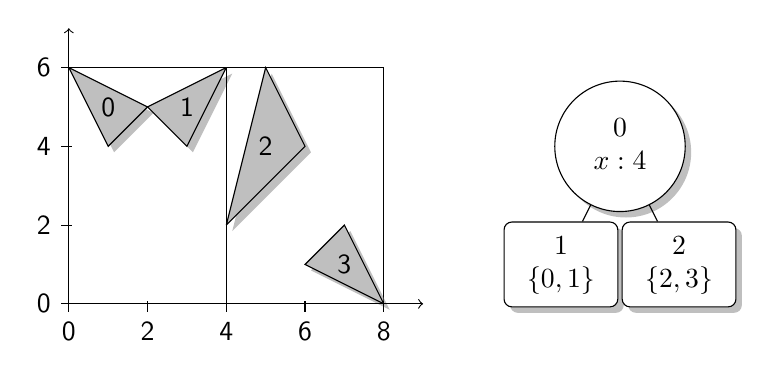
\begin{tikzpicture}[y=0.5cm, x=0.5cm,font=\sffamily]
      \drawNode{0,0}{8,0}{8,6}{0,6}
      
      % Tris
      \drawTri{0,6}{1,4}{2,5}
      \draw (1,5) node{0};
      \drawTri{4,6}{3,4}{2,5}
      \draw (3,5) node{1};
      \drawTri{4,2}{5,6}{6,4}
    \draw (5,4) node{2};
      \drawTri{8,0}{7,2}{6,1}
      \draw (7,1) node{3};

      % Splits
      \draw (4,0) -- (4,6);

      %axes
      \draw[->] (0,0) -- coordinate (x axis mid) (9,0);
      \draw[->] (0,0) -- coordinate (y axis mid) (0,7);
      %ticks
      \foreach \x in {0,2,...,9}
     		\draw (\x,1pt) -- (\x,-3pt)
			node[anchor=north] {\x};
      \foreach \y in {0,2,...,7}
     		\draw (1pt,\y) -- (-3pt,\y) 
     			node[anchor=east] {\y}; 

      \draw (14,4) node [node] (0){$\begin{array}{c}0\\x:4\end{array}$}
        child {node [leaf] (1) {$\begin{array}{c}1\\\{0, 1\}\end{array}$}}
        child {node [leaf] (2) {$\begin{array}{c}2\\\{2, 3\}\end{array}$}};
    \end{tikzpicture}
    \label{fig:simpleScene1}
  }
  \caption{One iteration of the kd-tree construction algorithm.}
  \label{fig:kdIteration}
\end{figure}


\subsection{Tree Representation}\label{sec:treeRepresentation}

Each interior node in a kd-tree must contain three pieces of information.

\begin{itemize}
\item \textit{Split axis} - The axis that an interior node is split
  along.
\item \textit{Split position} - The position of the splitting plane
  along the split axis.
\item \textit{Child references} - Information about how to find the
  node's children.
\end{itemize}

The first two items are pretty straightforward. The choice of axis, x,
y or z, can be stored inside two bits and the position of the splitting
plane should be stored as a floating point number. How an interior
nodes should reference its child nodes, however, is not as
straightforward.

% Left balanced non pointer vs pointers

In general there are two ways a node can reference its child
nodes. The first is through the use of \textit{balanced trees}, where
children of a node can be addressed implicitly without the use of
pointers. The reason for this is that nodes at the same tree level are
placed sequentially in memory and the start address of some tree
level, $l$ is given by $2^l-1$. The left and right child of node $n$
can then be indexed using $2n+1$ and $2n+2$. The parent of a node is
indexed with $\lceil n/2 \rceil - 1$.

% Balanced trees suck, example of partition with high density in one
% side and no triangles in other side. 

Wald et al.\citebook{wald:04:VVH} has the following to say about
balanced trees.

\quotebook{Balancing is optimal only for binary searching, and if all
  nodes have equal access probabilities. Neither of these two
  prerequisites are fulfilled for range queries (such as ray traversal
  and kNN queries), nor for unevenly distributed primitives such as
  photons or triangles.}{wald:04:VVH}

% Choose pointers as that would lead to less memory consumption and it
% places all nodes of the same level in a continues block, making it
% easier to work with them.

To avoid balanced trees we can instead use pointers to reference the
children. This allows for more flexibility when creating the tree. Unfortunately
it also means storing more data per node and in the case of slow memory access
it can cause a memory latency bottleneck. However, when experimenting with
different techniques for creating kd-trees, such as is done in this thesis, the
added flexibility can be a benefit. In \refsection{sec:gpuEmptySpace} we shall
see how this flexibility can be used to add the \textit{Empty Space Maximization}
optimization, without modifications to the existing kd-tree construction
implementation. This would not have been possible had the tree been balanced.

% Triangle references

The only information that must be stored in a kd-tree's leaf node is how to
reference the triangles associated with it. In this thesis I have choosen to
store a reference to the triangles associated with a leaf as one large list of
indices. I have adopted the convention that all triangle indices associated with
a given leaf must be stored sequentially in memory and a leaf therefore only
needs to contain a reference to its first triangle index and the amount of
triangles it is associated with. Using indices instead of actual triangles makes
it cheaper to perform sorting after a node has been split and its triangles have
been associated with its children. However to simplify the notation and keep the
algorithms simple, in the rest of the thesis I will assume that a leaf has
direct access to the triangles associated with it. When the number of triangles
associated with a node goes below a certain threshold I will switch the
representation to an index and a bit mask. How this will work and the advantages
of the bit mask representation will be explained in \refsection{sec:lowerNodes}.


\subsection{Choosing the Splitting Plane}\label{sec:splittingPlane}

% All the brilliance in KD-tree construction comes down to choosing the
% splitting plane and deciding when to stop.

Looking again at \refalg{alg:kdTreeCreator}, we can see that the brilliance
associated with constructing a high quality kd-tree is knowing where to place
the splitting plane and when to end the recursion and create a leaf.

% Different splitting planes heuristics.

In the following section I present two algorithms that solves this problem and
then I extend them with Empty Space Maximization, which will improve the quality
of the tree by allowing rays to quickly skip large subtrees and thus find the
geometry they intersect faster.


\subsubsection{Spatial Median}

% Split at the spatial median.

% Axis to split along can be choosen in a round robin fashion or the
% largest axis can be choosen. (Which initially minimises the surface
% of the children)

A quite simple method for choosing the splitting plane is to place it at the
spatial median of a node's bounding box. There are two ways to choose which
dimensions spatial median to use. A \textit{round robin} approach can be used,
where the dimensions are cycled every iteration; e.g. when creating the first
node the plane will lie perpendicular to the x-axis, that node's children will
then be split along the y-axis, in the next iteration the nodes will be split
along the z-axis and then the cycle restarts again at the x-axis. Another way of
choosing the dimension is to split along the largest axis of the node's bounding
box. This will be more costly than the round robin approach since more axes must
be analysed, but there is also a higher probability that it will produce trees
of higher quality.

The termination criteria for spatial median splitting is equally as simple as
choosing the splitting plane. If the number of triangles associated with a node
falls below a certain threshold, then that node becomes a leaf.

% Refered to as the naïve implementation in Wald07.

This method is refered to as naïve in \citebook{wald:06:NlogN} and rightly so,
since spatial median splitting does not take the distribution of geometry inside
a node's bounding box into account. On \reffig{fig:crapMedian} an example is
given where a node is split in a non-intuitive way. Spatial median splitting
does, however, make up for its suboptimal splitting planes by being quite fast.

 %% and I will therefore use it for creating my kd-trees upper nodes, as
 %% is described in \refsection{sec:upperNodes}.

\begin{figure}
  \centering
  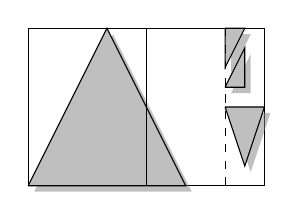
\begin{tikzpicture}[y=0.5cm, x=.5cm,font=\sffamily]
    % AABB
    \draw (0,0) -- (6,0) -- (6,4) -- (0,4) -- (0,0);

    % Tris
    \drawTri{0,0}{2,4}{4,0}
    \drawTri{5,4}{5.5,4}{5,3}
    \drawTri{5,2.5}{5.5,2.5}{5.5,3.5}
    \drawTri{5,2}{6,2}{5.5,0.5}

    % Split
    \draw (3,0) -- (3,4);
    \draw[dashed] (5,0) -- (5,4);

  \end{tikzpicture}

  \vspace{3mm}
  \parbox{5cm}{\caption[A poor split produced by median splitting.]{A poor split
      produced by median splitting. The solid line is a median split. The dashed
      one is a more optimal splitting plane, since it divides the large triangle
      from the small.}\label{fig:crapMedian}}
\end{figure}

\subsubsection{Surface Area Heuristic}\label{sec:SAH}

% SAH assumptions can be seen in Wald07

A far better splitting plane position can be obtained by applying the
\textit{Surface Area Heuristic}, \textit{SAH}. Instead of only considering the
bounding volume surrounding the geometry, SAH considers the entire geometry
associated with a node. In essence SAH computes the \textit{expected cost},
$C_{SAH}$, of traversing a node, $n$, that has been split into the child nodes
$l$ and $r$.

\begin{displaymath}
  C_{SAH}(n \rightarrow \{l, r\}) = C_{trav} + \frac{C_l A_l}{A_n} +
  \frac{C_r A_r}{A_n}
\end{displaymath}

where $C_{trav}$ is the cost of traversing an interior node and is independent
of the splitting plane, $C_l$ is the cost of traversing the left child node and
$C_r$ is the cost of traversing the right child node. $A_k$ is the summed
surface area of the geometry associated with node $k$. Choosing the most optimal
splitting plane amounts to applying SAH to all possible splitting planes and
then choosing the one with lowest cost. Since the above cost evaluation does not
take ray directions into account, SAH assumes that rays are uniformly
distributed, infinite lines.

% Globlly optimal is infeasable for complex scenes and instead a local
% greedy approximation is used.

SAH can also automatically determine when to stop splitting. The cost
of traversing a leaf node is given as

\begin{displaymath}
  C_{leaf}(n) = \|T_n\| C_i
\end{displaymath}

where $\|T_n\|$ is the number of triangles associated with $n$ and $C_i$ is the
cost of testing intersection between a triangle and a ray. SAH's termination
criteria is then $C_{leaf}(n) <= C_{SAH}(n)$, i.e. SAH terminates when the
expected cost of splitting $n$ becomes higher than the cost of keeping $n$ as a
leaf node.

Calculating a globally optimal solution using SAH is infeasable for complex
scenes, as that would require evaluating the cost of all possible subtrees. A
\textit{local greedy approximation} is used instead, where it is assumed that
the created child nodes are leafs. This assumption simplifies the SAH
calculation to

\begin{displaymath}
  C_{SAH}(n \rightarrow \{l, r\}) = C_{trav} + \frac{C_{leaf}(l) A_l}{A_n}
  + \frac{C_{leaf}(r) A_r}{A_n}
\end{displaymath}

The termination criteria can now be simplified into

\begin{displaymath}
  \begin{array}{rl}
    & C_{leaf}(n) <= C_{SAH}(n)\\
    \Updownarrow \\
    & \|T_n\| C_i <= C_{trav} + \frac{C_{leaf}(l) A_l}{A_n} + \frac{C_{leaf}(r)
      A_r}{A_n} \\
    \Updownarrow \\
    & \|T_n\| C_i <= C_{trav} + \frac{\|T_l\| C_i A_l}{A_n} + \frac{\|T_r\| C_i A_r}{A_n}\\
    \Updownarrow \\
    & A_n (\|T_n\| - \frac{C_{trav}}{C_i}) <=  \|T_l\| A_l + \|T_r\| A_r\\
  \end{array}
\end{displaymath}

Deciding on the optimal splitting plane is therefore reduced to finding the
plane with the least weighted area $\|T_l\| A_l + \|T_r\| A_r$ and choosing
appropriate values for the constants $C_{trav}$ and $C_i$ is reduced to
determining $C_{trav}/C_i$.

Inspite of the assumptions made by SAH about ray distribution and that in
practice a local greedy approximation is used, it is still considered one of the
best heuristics and can generally produces trees of the highest quality.

% SAH calculation optimizations include axis round robin and some damn
% paper I can't remember.


\paragraph{Split Candidates}

% To avoid having to test the infinitely many splitting planes
% possible, we instead have to choose sensible planes for SAH.

As mentioned above, the SAH cost needs to be evaluated for \textit{all}
available splitting planes. Since there are infinitely many potential planes
along either axis, some method is needed to distinguish the useful splitting
planes from unimportant ones. The interesting splitting planes are those
finitely many planes, where the geometry association in the resulting left and
right child nodes change. These splitting planes are called \textit{split
  candidates}.

%% and are \textit{tangent planes} to the geometry inside a node's bounding
%% volume. A tangent plane lies perpendicular to a geometric primitives surface
%% and only touches the surface of the triangle without intersecting it.

% Take planes from bounding volumes

The obvious choice of axis aligned split candidates are the 6 planes defined by
a triangle's axis aligned bounding box. These fulfil the requirement for
becoming split candidates, as they represent the exact location where the
geometry association for the left and right side changes. While using the
bounding box' sides is a simple and fast solution, it is not always the most
optimal. The reason for this is that a triangle may not be located entirely
inside a node and therefore its bounding box does not represent the most optimal
split. An example of this can be seen in \reffig{fig:aabbSplit}, where slightly
moving the split candidates given by the sides of the triangle's bounding box
would not change the triangle association in the resulting two leaf nodes.

\begin{figure}
  \centering
  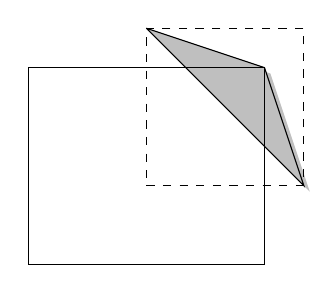
\begin{tikzpicture}[y=0.5cm, x=.5cm,font=\sffamily]

    % AABB
    \drawTri{3,6}{7,2}{6,5}
    \drawAabb{3,2}{7,2}{7,6}{3,6}

    \draw (0,0) -- (6,0) -- (6,5) -- (0,5) -- (0,0);
  \end{tikzpicture}

  \vspace{3mm}
  \parbox{5cm}{\caption[Triangle/Node bounding box intersection.]{An
      example of how the sides of a triangle's bounding box, the
      dashed box, does not represent the most optimal splitting
      planes.}\label{fig:aabbSplit}}
\end{figure}

Another problem with choosing the sides of a triangle's bounding box
as split candidates is that bounding boxes of small nodes may be
completely contained inside the geometry's bounding box. Thus none of
the planes are actually useful split candidates as they can not split
the node, which is demonstrated on \reffig{fig:aabbContained}.

\begin{figure}
  \centering
  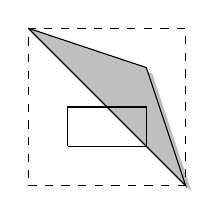
\begin{tikzpicture}[y=0.5cm, x=.5cm,font=\sffamily]

    \drawTri{0,4}{4,0}{3,3}
    \drawAabb{0,0}{4,0}{4,4}{0,4}

    % AABB
    \draw (1,1) -- (3,1) -- (3,2) -- (1,2) -- (1,1);

  \end{tikzpicture}
    
  \vspace{3mm}
  \parbox{5cm}{\caption[A tree node's bounding box contained in a
      triangle's bounding box.]{The kd-tree node's bounding box
      completely contained inside the triangles bounding
      box.}\label{fig:aabbContained}}
\end{figure}

A solution to this is to continuously \textit{clip} the bounding box of the
split geometry to fit the part of the geometry inside the tree nodes bounding
box, which creates optimal split candidates or \textit{perfect split
  condidates}, as demonstrated on \reffig{fig:aabbClipped}.

\begin{figure}
  \centering

  \subfloat[]{
    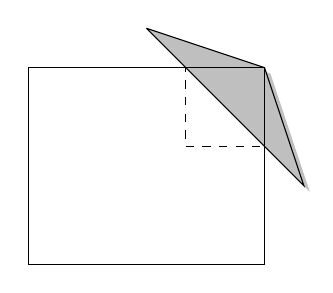
\begin{tikzpicture}[y=0.5cm, x=.5cm,font=\sffamily]
      
      % AABB
      \drawTri{3,6}{7,2}{6,5}
      \drawAabb{4,3}{6,3}{6,5}{4,5}

      \draw (0,0) -- (6,0) -- (6,5) -- (0,5) -- (0,0);
    \end{tikzpicture}
  }
  \hspace{5mm}
  \subfloat[]{
    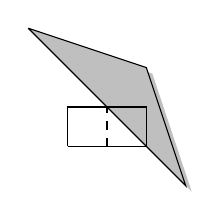
\begin{tikzpicture}[y=0.5cm, x=.5cm,font=\sffamily]

      \drawTri{0,4}{4,0}{3,3}
      \drawAabb{2,1}{2,2}{3,2}{3,1}

      % AABB
      \draw (1,1) -- (3,1) -- (3,2) -- (1,2) -- (1,1);

    \end{tikzpicture}
  }
  \hspace{5mm}
  \subfloat[]{
    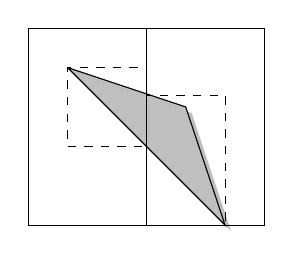
\begin{tikzpicture}[y=0.5cm, x=.5cm,font=\sffamily]
      
      \drawTri{0,4}{4,0}{3,3}
      \drawAabb{0,2}{2,2}{2,4}{0,4}
      \drawAabb{2,0}{4,0}{4,3.3}{2,3.3}
      
      % AABB
      \drawNode{-1,0}{2,0}{2,5}{-1,5}
      \drawNode{2,0}{5,0}{5,5}{2,5}

    \end{tikzpicture}
  }

  \vspace{3mm}
  \parbox{10cm}{ \caption[Triangle clipping.]{The triangles' bounding boxes have
      all been clipped to fit the part of the triangle contained in the nodes'
      bounding boxes.}\label{fig:aabbClipped}}
\end{figure}


\subsubsection{Empty Space Maximization}\label{sec:emptySpace}

An effective optimization to the quality of kd-trees is \textit{Empty Space
  Maximization} and it can be applied to both trees created with Spatial Median
Splitting or SAH. The idea behind the optimization is to cut away large empty
parts of the scene near the top of the tree. This is done by injecting empty
leaf nodes into the tree at interior nodes where the distance from their
parent's bounding box to the associated geometry is above a certain
threshold. The empty nodes will then provide rays traversing the tree with an
early out option, allowing them to skip a large portion of the geometry.

\Reffig{fig:noEmptySpaceExample} shows a simple scene without empty space cut
away and its corrosponding kd-tree. Without Empty Space Maximization the ray
entering the scene from the lower left cornor is forced to perform intersection
tests with every triangle in leaf 1. In contrast the kd-tree in
\reffig{fig:emptySpaceExample} has been created with Empty Space Maximization
enabled and the ray entering the scene now ends up in leaf 4. Leaf 4 is empty
and allows the ray to advance into the scene without testing for intersection
with any of the triangles in leaf 1.

\begin{figure}
  \centering
  \subfloat[A simple scene without empty space cut away.]{
    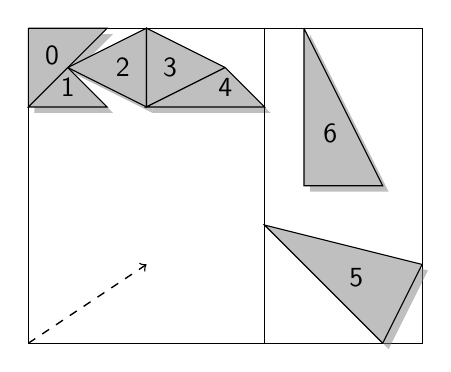
\begin{tikzpicture}[y=0.5cm, x=.5cm,font=\sffamily]
      
      % AABB
      \draw (0,0) -- (10,0) -- (10,8) -- (0,8) -- (0,0);
      
      % Tris
      \drawTri{9,0}{10,2}{6,3}
      \draw (8.33,1.66) node {5};
      \drawTri{7,8}{7,4}{9,4}
      \draw (7.67,5.33) node {6};
      
      \drawTri{0,8}{0,6}{2,8}
      \draw (0.6,7.3) node {0};
      \drawTri{1,7}{0,6}{2,6}
      \draw (1,6.5) node {1};
      \drawTri{1,7}{3,6}{3,8}
      \draw (2.4,7) node {2};
      \drawTri{5,7}{3,6}{3,8}
      \draw (3.6,7) node {3};
      \drawTri{5,7}{3,6}{6,6}
      \draw (5,6.5) node {4};
      
      % Splits
      \draw (6,0) -- (6,8);
      
      % Ray
      \drawRay{0,0}{3,2}
      
    \end{tikzpicture}
    \label{fig:noEmptySpaceScene}
  }
  \hspace{5mm}
  \subfloat[The tree corrosponding to the scene in \reffig{fig:noEmptySpaceScene}.]{
    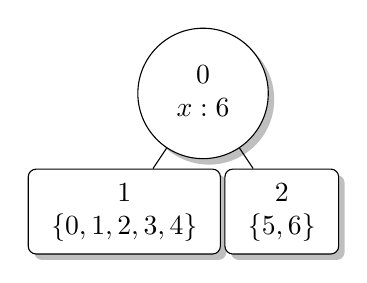
\begin{tikzpicture}[y=0.5cm, x=.5cm,font=\sffamily,
        level/.style={sibling distance=20mm/#1}]
      \node [node] {$\begin{array}{c}0\\x:6\end{array}$}
        child {node [leaf] {$\begin{array}{c}1\\\{0,1,2,3,4\}\end{array}$}}
        child {node [leaf] {$\begin{array}{c}2\\\{5, 6\}\end{array}$}};
    \end{tikzpicture}
    \label{fig:noEmptySpaceTree}
  }
  
  \caption[Scene without Empty Space Maximization.]{A kd-tree constructed around
    a simple scene. The kd-tree does not use the Empty Space Maximization
    optimization.}
  \label{fig:noEmptySpaceExample}
\end{figure}

\begin{figure}
  \centering
  \subfloat[The scene from \reffig{fig:noEmptySpaceScene} with empty space cut away.]{
    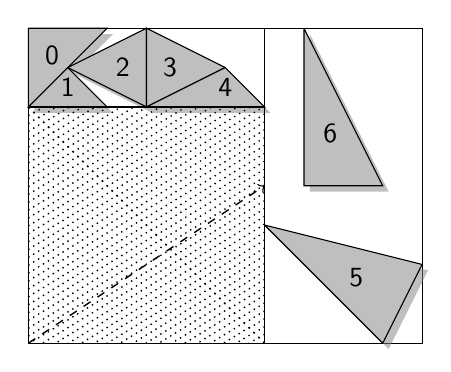
\begin{tikzpicture}[y=0.5cm, x=.5cm,font=\sffamily]
      
      % AABB
      \draw (0,0) -- (10,0) -- (10,8) -- (0,8) -- (0,0);
      
      % Tris
      \drawTri{9,0}{10,2}{6,3}
      \draw (8.33,1.66) node {5};
      \drawTri{7,8}{7,4}{9,4}
      \draw (7.67,5.33) node {6};
      
      \drawTri{0,8}{0,6}{2,8}
      \draw (0.6,7.3) node {0};
      \drawTri{1,7}{0,6}{2,6}
      \draw (1,6.5) node {1};
      \drawTri{1,7}{3,6}{3,8}
      \draw (2.4,7) node {2};
      \drawTri{5,7}{3,6}{3,8}
      \draw (3.6,7) node {3};
      \drawTri{5,7}{3,6}{6,6}
      \draw (5,6.5) node {4};
      
      % Splits
      \draw (6,0) -- (6,8);
      \draw (0,6) -- (6,6);
      
      % Empty space
%      \draw[ball color=gray, color=green, shading=ball,gray] (0,0) -- (0,6) -- (6,6) -- (6,0) -- (0,0);
      \foreach \x in {0,0.2,...,6}
        \draw[line width=0.5pt, dotted] (0, \x) -- (\x, 0);
      \foreach \x in {0,0.2,...,5.8}
        \draw[line width=0.5pt, dotted] (6, \x) -- (\x, 6);
      
      % Ray
      \drawRay{0,0}{6,4}
      
    \end{tikzpicture}
    \label{fig:emptySpaceScene}
  }
  \hspace{5mm}
  \subfloat[The tree from \reffig{fig:noEmptySpaceTree} with the empty space nodes 3 and 4 injected.]{
    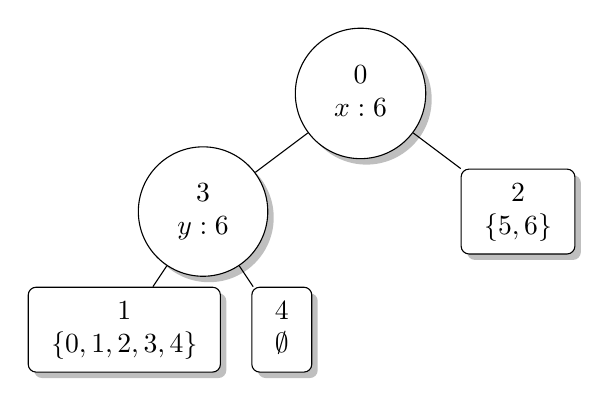
\begin{tikzpicture}[y=0.5cm, x=.5cm,font=\sffamily,
        level/.style={sibling distance=40mm/#1}]
      \node [node] {$\begin{array}{c}0\\x:6\end{array}$}
        child {node [node] {$\begin{array}{c}3\\y:6\end{array}$}
            child {node [leaf] {$\begin{array}{c}1\\\{0,1,2,3,4\}\end{array}$}}
            child {node [leaf] {$\begin{array}{c}4\\\emptyset\end{array}$}}
        }
        child {node [leaf] {$\begin{array}{c}2\\\{5, 6\}\end{array}$}};
    \end{tikzpicture}
    \label{fig:emptySpaceTree}
  }
  
  \caption[Empty Space Maximization.]{An example of Empty Space
    Maximization. The dotted region represents an empty node and allows the ray
    to leap across it, thus skipping intersection tests with the five triangles
    above.}\label{fig:emptySpaceExample}
\end{figure}


Unfortunately, the percentage of a node that should be empty space before it is
cut away is highly scene specific, making this optimization less usefull in the
general case. \zhou{} found that cutting away 25\% or more empty space produced
optimal trees, but instead of simply using their threshold I will test it with
threshold of 15\%, 25\% and 35\% in \refchapter{chp:results}.

% Dynamic empty space threshold, favor early out in the top of the tree.

% huge ray tracing performance improvement in testscene (23% without
% ray tracers doing intersection tests at leaf nodes)

% Implementation is 

\subsection{Triangle/Node Association Schemes}\label{sec:splittingSchemes}

When a splitting plane has been chosen, the interior node's associated triangles
needs to be associated with the child nodes whose bounding box they
overlap. Triangles located entirely in front of the splitting plane are
associated with the left child node and triangles entirely behind are associated
with the right child. The association schemes discussed in this section present
different methods for handling triangles intersected by the splitting plane. The
scheme employed is important in dynamic schemes. On one hand a fast
approximating association scheme may assign triangles to nodes that they do not
necessarily overlap, resulting in larger trees and thus slower ray tracing
times. On the other hand a scheme that rigorously checks every triangle and only
assigns triangles to nodes that they definitely overlap will result in a smaller
tree and faster ray tracing time, but will also incur a performance penalty when
constructing the acceleration structure.



\subsubsection{Triangle Splitting}

% Normally ppl split.

The most common approach when a triangle is intersected by a splitting plane, is
to split the triangle up into new triangles. New triangles produced by triangle
splitting will always be located entirely within the bounding box of the kd-node
they are associated with. When performing triangle splitting there are three
cases that must be handled, as can be seen in \reffig{fig:splittingCases}.

\begin{figure}
  \centering
  \subfloat[Two vertices to the left of the splitting plane.]{
    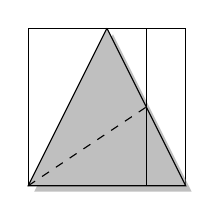
\begin{tikzpicture}[y=0.5cm, x=.5cm,font=\sffamily]
      \draw (0,0) -- (4,0) -- (4,4) -- (0,4) -- (0,0);
      \drawTri{2,4}{0,0}{4,0}
      \draw[dashed] (0,0) -- (3,2);
      \draw (3,0) -- (3,4);
    \end{tikzpicture}
    \label{fig:splittingCase1}
  }
  \hspace{5mm}
  \subfloat[One vertex intersected by the splitting plane.]{
    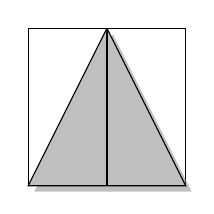
\begin{tikzpicture}[y=0.5cm, x=.5cm,font=\sffamily]
      \draw (0,0) -- (4,0) -- (4,4) -- (0,4) -- (0,0);
      \drawTri{2,4}{0,0}{4,0}
      \draw (2,0) -- (2,4);
    \end{tikzpicture}
    \label{fig:splittingCase2}
  }
  \hspace{5mm}
  \subfloat[Two vertices to the right of the splitting plane.]{
    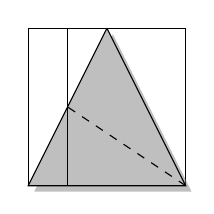
\begin{tikzpicture}[y=0.5cm, x=.5cm,font=\sffamily]
      \draw (0,0) -- (4,0) -- (4,4) -- (0,4) -- (0,0);
      \drawTri{2,4}{0,0}{4,0}
      \draw[dashed] (4,0) -- (1,2);
      \draw (1,0) -- (1,4);
    \end{tikzpicture}
    \label{fig:splittingCase3}
  }

  \vspace{3mm}
  \parbox{10cm}{\caption[The three different triangle splitting
      cases.]{The three different triangle splitting cases. A dashed
      line represents an additional split needed to keep representing
      geometry as triangles.}\label{fig:splittingCases}}
\end{figure}

The first case in \reffig{fig:splittingCase1} illustrates the split when two
vertices are located on the left of the splitting plane and one on the
right. This case is mirrored by \reffig{fig:splittingCase3} where two of the
vertices are located to the right of the splitting plane. In both of these cases
a triangle split will produce three new triangles. The last case in
\reffig{fig:splittingCase2} shows one of the vertices located inside the
splitting plane and splits the triangle perfectly into two new triangles. This
last case however is highly unlikely and in general it can be assumed that a
split triangle always produces three new triangles.


\subsubsection{Triangle/Node Overlap}

\begin{figure}
  \centering
  \subfloat[One split.]{
    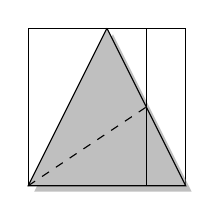
\begin{tikzpicture}[y=0.5cm, x=0.5cm,font=\sffamily]
      \draw (0,0) -- (4,0) -- (4,4) -- (0,4) -- (0,0);
      \drawTri{2,4}{0,0}{4,0}
      \draw[dashed] (0,0) -- (3,2);
      \draw (3,0) -- (3,4);
    \end{tikzpicture}
  }
  \subfloat[Two splits.]{
    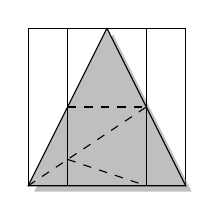
\begin{tikzpicture}[y=0.5cm, x=0.5cm,font=\sffamily]
      \draw (0,0) -- (4,0) -- (4,4) -- (0,4) -- (0,0);

      \drawTri{2,4}{0,0}{4,0}
      
      \draw (1,0) -- (1,4);
      \draw (3,0) -- (3,4);

      \draw[dashed] (1,2) -- (3,2);
      \draw[dashed] (0,0) -- (3,2);
      \draw[dashed] (1,0.667) -- (3,0);
    \end{tikzpicture}
  }
  \subfloat[Three splits.]{
    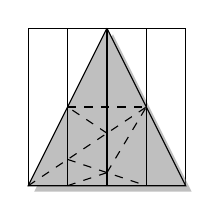
\begin{tikzpicture}[y=0.5cm, x=0.5cm,font=\sffamily]
      \draw (0,0) -- (4,0) -- (4,4) -- (0,4) -- (0,0);
      \drawTri{2,4}{0,0}{4,0}
      
      \draw (1,0) -- (1,4);
      \draw (2,0) -- (2,4);
      \draw (3,0) -- (3,4);

      \draw[dashed] (1,2) -- (3,2);
      \draw[dashed] (0,0) -- (3,2);
      \draw[dashed] (1,0.667) -- (3,0);
      \draw[dashed] (2,0.333) -- (1,0);
      \draw[dashed] (2,0.333) -- (3,2);
      \draw[dashed] (2,1.333) -- (1,2);
    \end{tikzpicture}
  }

  \vspace{3mm}
  \parbox{8cm}{\caption[Excessive splitting of a triangle.]{The triangle splitting
      algorithm performing excessive splits on a triangle.}\label{fig:excessiveSplitting}}
\end{figure}

Since splitting a triangle almost always leads to three new triangles being
created, this can result in excessively many new triangles, as evidenced by
\reffig{fig:excessiveSplitting} where the same triangle is split three
times. The problem with excessive splitting is that each new triangle actually
represents the original triangle and on \reffig{fig:excessiveSplitting} nodes
can be seen containing up to 6 triangles, which all represents the exact same
original and are cluttering up the tree with redundant geometry. A more
preferable situation is seen in \reffig{fig:dividing}, where each leaf node only
contains one reference to the original triangle.

\begin{figure}
  \centering
  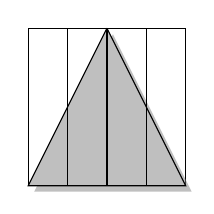
\begin{tikzpicture}[y=0.5cm, x=0.5cm,font=\sffamily]
    \draw (0,0) -- (4,0) -- (4,4) -- (0,4) -- (0,0);
    \drawTri{2,4}{0,0}{4,0}
    
    \draw (1,0) -- (1,4);
    \draw (2,0) -- (2,4);
    \draw (3,0) -- (3,4);
  \end{tikzpicture}
  
  \vspace{3mm}
  \parbox{5cm}{\caption[Dividing a triangle.]{Dividing a triangle among the
      leafs associated with it. Notice that each leaf only contains one
      reference to the original triangle.}\label{fig:dividing}}
\end{figure}

This is the central idea behind performing a \textit{Triangle/Node Overlap}
test. Instead of splitting a triangle by the splitting plane and creating new
triangles, the original triangle is associated with a leaf node if the triangle
and the leaf node's bounding box overlap. How to test this is described in
Möller\citebook{Moller:2005}.

%% Whether or not to associate a triangle and node is decided by performing a
%% \textit{triangle/bounding box overlap} test, as described in
%% Möller\citebook{Moller:2005}. If the triangle overlaps the leaf node's
%% bounding box after the split, then it will be associated with that node,
%% otherwise the triangle will not be a part of that nodes geometry.


\subsubsection{Box Inclusion}\label{sec:boxInclusion}

% Simpler than splitting.

Performing a triangle/bounding box overlap test required for Triangle/Node
Overlap can be a computationally heavy task. A cheaper splitting scheme is to
test if the triangle's axis aligned bounding box, $t$, overlaps with the axis
aligned bounding box of the node, $n$. Performing the overlap test between these
axis aligned bounding boxes is simply

\begin{displaymath}
  \text{overlap}(n,t) = n_{min} < t_{max} \wedge t_{min} < n_{max}
\end{displaymath}

where the infix operator $<: \{R^3, R^3\} \rightarrow bool$ is defined as $n < t
= n.x < t.x \wedge n.y < t.y \wedge n.z < t.z$.

\begin{figure}
  \centering \subfloat[Box Inclusion correctly associates the triangle to both
    nodes.]{
    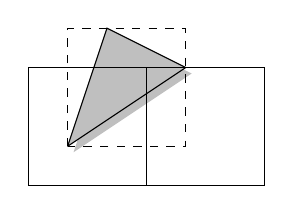
\begin{tikzpicture}[y=0.5cm, x=.5cm] 
      \drawTri{1,1}{2,4}{4,3}
      \drawAabb{1,1}{1,4}{4,4}{4,1}
      
      \draw (0,0) -- (0,3) -- (3,3) -- (3,0) -- (0,0);
      \draw (3,0) -- (3,3) -- (6,3) -- (6,0) -- (3,0);
    \end{tikzpicture}
  }
  \hspace{5mm}
  \subfloat[Box Inclusion will incorrectly associate the the triangle with the
    left node.]{
    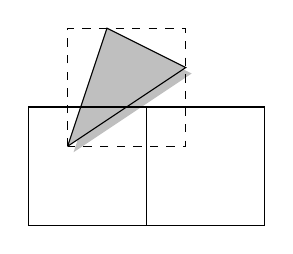
\begin{tikzpicture}[y=0.5cm, x=.5cm]
      \drawTri{1,2}{2,5}{4,4}
      \drawAabb{1,2}{1,5}{4,5}{4,2}

      \draw (0,0) -- (0,3) -- (3,3) -- (3,0) -- (0,0);
      \draw (3,0) -- (3,3) -- (6,3) -- (6,0) -- (3,0);
    \end{tikzpicture}
    \label{fig:falseBoxInclusion}
  }
  \caption{Box inclusion examples.}
  \label{fig:boxInclusion}
\end{figure}

% Naturally increases amount of \textit{false primitives} in the tree, but is
% very cheap.

\Reffig{fig:boxInclusion} shows two examples of a node being split down the
middle. In both examples the triangle will be associated with both new nodes, as
the triangle's bounding box overlaps both nodes. But in
\reffig{fig:falseBoxInclusion} we clearly see that the triangle itself does not
overlap the right node's bounding box. This illustrates the drawback of only
testing a triangle's bounding box and how Box Inclusion can produce
\textit{false positives}, where geometric primitives are associated with nodes
they do not overlap. Such false postives will increase the size of the tree and
thus slow down ray tracers. However, Box Inclusion makes up for this by
performing fast node/triangle association, cutting down on the time spent
constructing the tree.



% Also has an increased change of looping during construction in
% combination with a small max lower size. Fx fairy forest loops using
% adjusting bounding box with a max size of 32 primtives in leaf nodes.

% False primitives can then be removed at a later stage at the cost of
% some extra overhead. Or combine with Divide every n'th step for
% optimal sweetness.

% With the added leaf intersection in the ray tracer, extra triangles
% in the leaf nodes become even less important and this method starts
% to shine for dynamic scenes.




\section{Adopting the Algorithms for CUDA}\label{sec:kdTreeImpl}

% Needs to exploit the dataparallel nature of GPU's A GPU needs as many of its
% multiprocessors occupied as possibly for optimal performance.

Having explored the different methods for deciding which splitting plane to use
and how to associate geometry with a node in the kd-tree, it is time to look at
the actual implementation of a kd-tree construction algorithm on the GPU.

The general kd-tree construction method presented in \refalg{alg:kdTreeCreator}
recursively constructs \textit{one} tree node at a time in a
\textit{depth-first} manor. In order to efficiently utilize the GPU, as many of
its multiprocessors as possible must be fully occupied. This means that
\refalg{alg:kdTreeCreator} must be restructured to work on multiple nodes in
parallel. Fortunately this is exactly what \zhou{} did by changing the kd-tree
constructor to work on a list of nodes and recursively create the tree in
\textit{breadth-first} order, as outlined in \refalg{alg:bfsKDTreeCreator}.

\begin{algorithm}
  \caption{BFS recursive kd-tree constructor}
  \label{alg:bfsKDTreeCreator}
  \begin{algorithmic}
    \PROCEDURE{CreateNodes}
              {$activeNodes$ : Node List  \textit{\color{gray}//list of kd-nodes not processed yet}}
              {$nextNodes$ : Node List}
              {\PARALLELFOR{$node$}{$activeNodes$}
                 \IF{IsLeaf($node$)}
                   \ASSIGN{$node$}{Leaf($node$)}
                 \ELSE
                   \COMMENTIT{Determine the splitting plane.}
                   \ASSIGN{$plane$}{DeterminePlane($node$)}
                   \ASSIGN{$(node_L, node_R)$}{Split($node, plane$)}
                   \COMMENTIT{Associate the geometry with a node and add it to the next list.}
                   \ASSIGN{$node_L.geometry$}{AssociateGeometry($node.geometry, node_L$)}
                   \STATE{$nextNodes$.Add($node_L$)}
                   \ASSIGN{$node_R.geometry$}{AssociateGeometry($node.geometry, node_R$)}
                   \STATE{$nextNodes$.Add($node_R$)}
                 \ENDIF
               \ENDFOR}
  \end{algorithmic}
\end{algorithm}

% Creating the KD-tree in BFS will optimize GPU performance at lower tree
% levels, as there would be thousands of nodes created at the same time.

At the bottom levels, where thousands of nodes are created in parallel,
breadth-first creation allows full utilization of the GPU. But for the upper
levels of the tree this approach will still not fully exploit the graphics
hardware, as only a couple of nodes are active per iteration, leaving the
multiprocessors underutilized.

To remedy this the tree construction will be split into two phases, an upper and
a lower phase. A node is said to belong to the upper part of the tree if the
number of triangles associated with it is above a given threshold. In this
thesis I will be using the thresholds 32 and 64. During the upper tree creation
phase, the choice of splitting plane is parallelized over all geometric
primitives, of which there can be hundreds of thousands. When creating the lower
tree, there will be thousands of nodes and computations can effectively be
structured as in \refalg{alg:bfsKDTreeCreator}.

% The structure of the rest of the chapter.

The overall construction of the tree is presented in
\refalg{alg:constructKDTree}. First the axis aligned bounding box for each
triangle is precomputed. These are used to effectively compute the bounding
boxes of nodes and for Box Inclusion, if that association scheme is used. Then
the upper part of the tree is constructed iteratively until there are no more
new nodes to process. How this is achieved is the topic of
\refsection{sec:upperNodes}. Once the upper part of the tree is constructed, the
leaf nodes are processed to prepare for the lower tree construction phase. The
lower part of the tree is then iteratively constructed and
\refsection{sec:lowerNodes} details three different algorithms that produces
lower trees with varying construction speed and quality.

\begin{algorithm}
  \caption{Construct kd-tree}
  \label{alg:constructKDTree}
  \begin{algorithmic}
    \PROCEDURE{ConstructKDTree}
              {$Triangles$ : Triangle List}
              {$root$ : Node}{
                \PARALLELFOR{$t$}{$Triangles$}
                  \STATE{Compute axis aligned bounding box for $t$.}
                \ENDFOR
                \STATE{}
                \DECLARE{$activeNodes, leafs, nextNodes$}{Node List}
                \COMMENTIT{Upper node construction phase.}
                \STATE{$activeNodes$.Add($rootNode$)}
                \WHILE{$activeNodes$.NotEmpty}
                  \STATE{$nextNodes$.Clear}
                  \ASSIGN{$(newLeafs, nextNodes)$}{CreateUpperNodes($activeNodes$)}
                  \STATE{$leafs$.Append$(newLeafs)$}
                  \STATE{swap($activeNodes$, $nextNodes$)}
                \ENDWHILE
                \STATE{}
                \COMMENTIT{Lower node construction phase.}
                \STATE{PreprocessLowerNodes($leafs$)}
                \STATE{CreateLowerNodes($leafs$, $activeNodes$)}
                \WHILE{$activeNodes$.NotEmpty}
                  \STATE{$nextNodes$.Clear}
                  \ASSIGN{$nextNodes$}{CreateLowerNodes($activeNodes$)}
                  \STATE{swap($activeNodes$, $nextNodes$)}
                \ENDWHILE
              }
  \end{algorithmic}
\end{algorithm}

\subsection{Upper Tree Creation}\label{sec:upperNodes}

% At upper tree level nodes exploit data parallelism by parallelizing the cost
% computation over triangles.

At the uppermost levels of the kd-tree there will not be many nodes over which
computations can be parallelized. But each node can be associated with thousands
of geometric primitives and parallelizing the choice of splitting plane across
the geometry will utilize the GPU effectively.

% SAH assumes that each split results in two leaf nodes, which is practically
% always wrong at high level nodes, therefore \zhou{} suggests splitting along
% the spatial median of the nodes longest axis.

The issue is then which algorithm to use when choosing the splitting plane. The
Surface Area Heuristic provides an algorithm that can easily be parallelized
over the geometry. Each triangle would then be responsible for computing the
expected cost of splitting a node with its 6 bounding box planes and afterwards
the best possible plane could be reduced with the method described in
\refsection{sec:reduce}. Unfortunately there can be hundreds of thousand of
triangles associated with the tree's upper nodes, so comparing a split candidate
with all of them becomes computationally heavy. SAH also assumes that the created
children will be leaf nodes in the final tree and therefore that their cost can
be computed using $C_{leaf}$, which is almost never true at the top of the
tree. This makes SAH an undesirable algorithm for choosing splitting planes for
the upper tree, since we need to be able to decide on which splitting plane to
use fast to accomodate dynamic scenes. Instead \zhou{} proposes to use spatial
median splitting with Empty Space Maximization. Parallizing the splitting plane
decision over the geometry then becomes reducing an axis aligned bounding box
from a node's associated triangles, again as described in
\refsection{sec:reduce}, and then each node can use that bounding box to decide
where to place its splitting plane.

To associate triangles and nodes in the upper parts of the tree, both schemes
described in \refsection{sec:splittingSchemes} can be employed. As with the
splitting plane decision, the triangle/node association scheme will be
parallelized over all triangles. Since I have made the assumption that all
triangles associated with a node must be placed sequentially in memory, the
triangles need to be sorted after the triangle/node association has been
determined. To parallelize this sorting over all triangels, I again make use of
the scan primitive described in \refsection{sec:GPUprims}. Since a triangle can
be associated with both child nodes, the left-right sorting in
\refsection{sec:GPUprims} is not directly applicable. Instead I will be using a
variant where the prefix-sum calculation is applied to a list, $associateSide$,
of size $2 \cdot \|triangles\|$. In the first half of $associateSide$ I will
then use 0's and 1's to represent whether the $t$'th triangle overlapped its
current node's left child. In the last half of the list the same is done but for
the right child instead. Computing the prefix-sum of this list then yields the
addresses, $associateAddr$, where the triangles should be copied to. Below is an
example of this

\begin{displaymath}
  \begin{array}{r c c c c c c c c c c c c c}
    triangles: & [t_0 & t_1 & t_2 & t_3 & t_4 & t_5] & \color{lightgray}[t_0 & \color{lightgray}t_1 & \color{lightgray}t_2 & \color{lightgray}t_3 & \color{lightgray}t_4 & \color{lightgray}t_5]\\
    associateSide: & [1 & 1 & 0 & 1 & 1 & 0 & 1 & 0 & 1 & 0 & 0 & 1]\\
    associateAddr: & [0 & 1 & 2 & 2 & 3 & 4 & 4 & 5 & 5 & 6 & 6 & 6 & 7]\\
    sorted: & [t_0 & t_1 & t_3 & t_4 & t_0 & t_2 & t_5]
  \end{array}
\end{displaymath}

where the $triangles$ list is duplicated to easily show the association between
the entries in $associateSide$ and the triangles. With the $associateSide$ and
$associateAddr$ lists it is possible to parallelize the triangle sorting
effectively over all triangles using the algorithm in \refalg{alg:triangleSort}.

\begin{algorithm}
  \caption{Parallel triangle sorting.}
  \label{alg:triangleSort}
  \begin{algorithmic}
    \PROCEDURE{TriangleSort}
              {$triangles$ : Triangle List, $associateSide$ : Bit List, $associateAddr$ : Integer List}
              {$sorted$ : Triangle List}
              {\DECLARE{$sorted$}{Triangle List}
                \PARALLELFOR{$t$}{$triangles$}
                \IF{$associateSide$[$t$]}
                  \ASSIGN{$addr$}{$associateAddr$[$t$]}
                  \ASSIGN{$sorted$[$addr$]}{$t$}
                \ENDIF
                \IF{$associateSide$[$t + \|triangles\|$]}
                  \ASSIGN{$addr$}{$associateAddr$[$t + \|triangles\|$]}
                  \ASSIGN{$sorted$[$addr$]}{$t$}
                \ENDIF
               \ENDFOR}
  \end{algorithmic}
\end{algorithm}

% Explain the overall strcuture, how the last n nodes are active
% nodes?

\begin{figure}
  \centering
  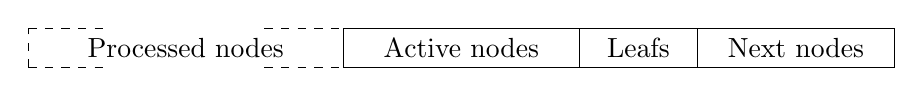
\begin{tikzpicture}[y=0.5cm, x=0.5cm]
    \draw[dashed] (0,1) -- (2,1);
    \draw[dashed] (0,0) -- (0,1);
    \draw[dashed] (0,0) -- (2,0);
    \draw (4,0.5) node {Processed nodes};
    \draw[dashed] (6,1) -- (8,1);
    \draw[dashed] (6,0) -- (8,0);
    \draw (8,1) -- (8,0);

    \draw (8,1) -- (22,1);
    \draw (8,0) -- (22,0);

    \draw (11,0.5) node {Active nodes};
    \draw (14,1) -- (14,0);

    \draw (15.5,0.5) node {Leafs};
    \draw (17,1) -- (17,0);

    \draw (19.5,0.5) node {Next nodes};
    \draw (22,1) -- (22,0);

  \end{tikzpicture}
  \caption{The structure of the kd-trees nodes in memory.}
  \label{fig:nodeStructure}
\end{figure}

%\fixme{Place this somewhere else?}

Like the triangles, the nodes themselves are placed in one large array with the
structure shown in \reffig{fig:nodeStructure}. The already processed nodes are
placed in one sequential chunk from index 0. The currently active nodes are
located right after them. The child nodes created by
\refalg{alg:kdUpperNodeCreator} are then placed after the active nodes, with the
leaf nodes to the left and next set of active nodes to the right. This preserves
the invariant that the $n$ currently active nodes, if any, are always the $n$
last nodes in the array after an iteration of the construction algorithm. This
is a desirable property as it means I do not need to maintain a list of indices
to active nodes, but can instead describe the list $activeNodes$ by a range and
an index into the node list. This also improves coalescence when subsequent
threads can access nodes sequentially.


\begin{algorithm}
  \caption{KD-Tree upper node creator}
  \label{alg:kdUpperNodeCreator}
  \begin{algorithmic}
    \PROCEDURE{CreateUpperNodes}
               {\VAR{activeNodes} : Node List}
               {\VAR{leafs,nextNodes} : Node List}{
                 \COMMENTIT{First split all triangles into segments.}
                 \DECLARE{$segmentList$}{List}
                 \PARALLELFOR{$node$}{$activeNodes$}
                   \STATE{Split all triangles contained in $node$ into
                     fixed sized segments and store those in $segmentList$.}
                 \ENDFOR
                 \STATE{}
                 \COMMENTIT{Then compute each triangles bounding box
                   using reduction as described in
                   \refsection{sec:reduce}.}
                 \PARALLELFOR{$segment$}{$segmentList$}
                   \STATE{Compute the bounding box of the triangles in
                     each segment.}
                 \ENDFOR
                 \STATE{Use segmented reduction as described in
                   \zhou{} to compute each nodes bounding box.}
                 \PARALLELFOR{$node$}{$activeNodes$}
                   \STATE{Split $node$ along its spatial median.}
                 \ENDFOR

                 \STATE{}
                 \COMMENTIT{Perform Empty Space Maximization.}
                 \COMMENTIT{See \refalg{alg:emptySpaceMaximization}.}
                 \STATE{...}
                 \STATE{}

                 \COMMENTIT{Compute the addresses to sort the
                   triangles to by comparing them to the splitting
                   plane.}
                 \DECLARE{$associateSide, associateAddr$}{List}
                 \PARALLELFOR{$segment$}{$segmentList$}
                   \PARALLELFOR{$triangle$}{$segment.triangles$}
                     \ASSIGN{$associateSide[triangle.id]$}{AssociateLeft($segment.node$, $triangle$)}
                     \ASSIGN{$associateSide[triangle.id + \|triangles\|]$}{AssociateRight($segment.node$, $triangle$)}
                   \ENDFOR
                 \ENDFOR
                 \ASSIGN{$associateAddr$}{\textbf{Prefix-Sum}($associateSide$)}
                 \COMMENTIT{Sort the triangles.}
                 \ASSIGN{$triangles$}{TriangleSort$(triangles, associateSide, associateAddr)$}
                 %% \PARALLELFOR{$segment$}{$segmentList$}
                 %%   \PARALLELFOR{$triangle$}{$segment.triangles$}
                 %%     \STATE{Sort the triangles to have triangles
                 %%       associated with the same node placed
                 %%       sequentially.}
                 %%   \ENDFOR
                 %% \ENDFOR

                 \STATE{}

                 \COMMENTIT{Split nodes.}
                 \PARALLELFOR{$node$}{$activeList$}
                   \STATE{Split the nodes into child
                     nodes. $associateSide$ and $associateAddr$ is
                     used to directly calculate the child nodes
                     triangle index and range.}
                   \COMMENTIT{Sort child nodes into the leaf and nextNodes
                     list. This is achieved just like the example from
                     \refsection{sec:GPUprims}.}

                   \IF{$node.child$.size < $threshold$}
                     \STATE{$leaf$.Add($node.child$)}
                   \ELSE
                     \STATE{$nextNodes$.Add($node.child$)}
                   \ENDIF
                 \ENDFOR
  }
  \end{algorithmic}
\end{algorithm}

% Go over the algorithm

The algorithm for constructing the upper parts of the kd-tree can be
seen in \refalg{alg:kdUpperNodeCreator}. It takes a list of non
processed nodes, $activeNodes$ as input and returns a list of leaf
nodes, $leafs$, and a list of new nodes, $nextNodes$, that needs to be
processed in the next iteration.


% Use GPU for computations and let CPU handle minor book keeping.

The first thing that \refalg{alg:kdUpperNodeCreator} does is split the triangles
associated with each active node into fixed-size segments. This may seem odd at
first, but recall that the upper nodes are split along the spatial median, that
finding the spatial median means computing a tight bounding box around the
geometry associated with a node, and that to do this we need to apply the
reduction described in \refsection{sec:reduce}. Generally having fixed-size
segments will also make it easier to choose a kernels block size, so that each
segment is processed by one block. A segment contains information about which
triangles it contains, which node its triangles are associated with and, incase
there are not enough triangles to fill it, it also stores how many triangles it
actually contains. The reduction kernel can use this information to pad the data
loaded into shared memory with identity elements.

After having segmented the triangles, the bounding boxes of the individual
segments can be computed as shown in \refsection{sec:reduce} by using the
operators \textbf{min} and \textbf{max} with their identity elements.
Performing a segmented reduction on the result, as described in Algorithm 3 in
\zhou, will then compute a tight bounding box for each node in activeList. A
kernel working on all active nodes will then use this bounding box to place the
nodes splitting planes along their spatial median.

With the splitting plane determined for each node, the triangles will be able to
determine their triangle/node association with the nodes children and sort
themselves into a new list as described above.

%% Instead of reducing the sizes of child nodes, as done in \zhou{} I propose a
%% method for calculating them directly. This leads to lots of uncoalesced
%% lookups, so argue if the GPU is able to properly hide these.

Lastly the nodes in $activeList$ are split into their child nodes in
parallel. For node $n$, the values in $associateAddr$ can be used to calculate
the triangle index and range of the child nodes, $left$ and $right$, as seen in
\refalg{alg:childIndices}. The idea behind \refalg{alg:childIndices} is that
using the triangle index of the parent nodes we are able to extract the triangle
index of its left and right child nodes. Then by adding the number of triangles
in the parent node to its index, we can lookup the starting index of the next
child node's triangles. Subtracting these two values yields the range of
triangles spanned by a child node.

\begin{algorithm}
  \caption{Compute child node triangle index and range}
  \label{alg:childIndices}
  \begin{algorithmic}
    \PROCEDURE{ChildTriangleInformation}
              {$parent, left, right$: Node, $associateAddr$ : List}
              {$left$ : Node, $right$ : Node}{
                \ASSIGN{$left.triangleIndex$}{$associateAddr[parent.triangleIndex]$}
                \ASSIGN{$leftEndAddr$}{$associateAddr[parent.triangleIndex + parent.triangleRange]$}
                \ASSIGN{$left.triangleIndex$}{$leftEndAddr - left.triangleIndex$}
                \ASSIGN{$right.triangleIndex$}{$associateAddr[parent.triangleIndex + \|triangles\|]$}
                \ASSIGN{$rightEndAddr$}{$associateAddr[parent.triangleIndex + parent.triangleRange]$}
                \ASSIGN{$right.triangleIndex$}{$rightEndAddr - right.triangleIndex$}
              }
  \end{algorithmic}
\end{algorithm}



% Building the upper nodes mostly consist of moving data around, and
% not necessarily in a coalesced fashion. This makes it hard to hide
% the latency and will impact performance.

% Argue it can be done in O ( N log N )



\subsubsection{Adding Empty Space Maximization}\label{sec:gpuEmptySpace}

% Plugable solution, add the new nodes after the ones in nextlist.

To experiment with the Empty Space Maximization optimization it needs to be
implemented as a solution that can be turned on and off at will. This has been
achieved with the design found in \refalg{alg:emptySpaceMaximization}, which
injects new nodes created by Empty Space Maximization into the tree. In order for
a node to perform Empty Space Maximization it needs a \textit{loose bounding
  box}. The loose bounding box is computed by splitting a parents bounding box
with its splitting plane. Since the geometry inside a child might not touch all
sides of a parents bounding box, the loose bounding box provides a loose upper
bound on the geometry associated with a child.

\begin{algorithm}
  \caption{Calculate Empty Space Maximization}
  \label{alg:emptySpaceMaximization}
  \begin{algorithmic}
    \PROCEDURE{CreateUpperNodes}
               {\VAR{activeNodes} : Node List}
               {\VAR{leafs,nextNodes} : Node List}{

                 \COMMENTIT{First split all triangles into segments.}
                 \STATE{...}
                 \COMMENTIT{Then compute each triangles bounding box
                   using reduction as described in
                   \refsection{sec:reduce}.}
                 \STATE{...}

                 \STATE{}
                 \COMMENTIT{Perform Empty Space Maximization.}
                 \IF{$performEmptySpaceMaximization$}
                 \DECLARE{$emptySplitNodes, emptyAddr$}{List}
                 \DECLARE{$emptySides$}{Plane List}
                 \PARALLELFOR{$node$}{$activeList$}
                 \ASSIGN{$emptySplits[i]$}{$0$}
                   \FOREACH{$side$}{$node.boundingBox$}
                     \IF{$node$ has more than $C_e$ empty space on $side$}
                       \ASSIGN{$emptySplitNodes[i]$}{$emptySplitNodes[i] + 2$}
                       \STATE{$emptySides[node]$.Add($side$)}
                     \ENDIF
                   \ENDFOR
                 \ENDFOR
                 \ASSIGN{$emptyAddr$}{\textbf{Prefix-Sum}($emptySplitNodes$)}
                 \PARALLELFOR{$node$}{$activeList$}
                   \STATE{Cut of empty space of sides in $emptySides$ and place
                     new nodes sequentially at addresses specified in
                     $emptyAddr$. Then rewire parent nodes to point to new
                     nodes.}
                 \ENDFOR
                 \ENDIF

                 \STATE{}
                 \COMMENTIT{Compute the addresses to move the
                   triangles to by comparing them to the splitting
                   plane.}
                 \STATE{...}
                 \COMMENTIT{Move the triangles.}
                 \STATE{...}

                 \COMMENTIT{Split nodes.}
                 \STATE{...}
  }
  \end{algorithmic}
\end{algorithm}

% Explain

The algorithm for performing Empty Space Maximization is inserted into
\refalg{alg:kdUpperNodeCreator} right after computing the nodes' tight bounding
boxes and before the new child nodes are created. Whether or not Empty Space
Maximization should be performed on any of the nodes in $activeNodes$ is then
checked in parallel for all nodes. The sides of a node's bounding box is checked
sequentially to see if the empty space between the loose and the tight bounding
box is above a certain threshold, which means that the empty space should be cut
away. These sides are added to the list $emptySides$, which will be used later
when the nodes are split. Each such split results in two new nodes, one node
that refers to the empty space and one node injected between the parent node and
its child node in active list. This injection is depicted in
\vreffig{fig:noEmptySpaceExample} and \vreffig{fig:emptySpaceExample}. The
number of new nodes created per node in $activeList$ by performing Empty Space
maximization is stored in $emptySplitNodes$.

Once the sides that should have empty space cut away has been determined, where
to place the nodes created by these splits are computed by calculating the
prefix-sum of $emptySplitNodes$. Empty Space Maximization nodes are injected
into to the list of nodes shown in \reffig{fig:nodeStructure} as described on
\reffig{fig:emptyNodeStructure}, which again preserves the invariant that the
next batch of active nodes are located at the end of the list. The arrows in
\reffig{fig:emptyNodeStructure} symbolize the parent$\rightarrow$child
relationship and very accuratly show how the new nodes are injected into the
tree.

\begin{figure}
  \centering
  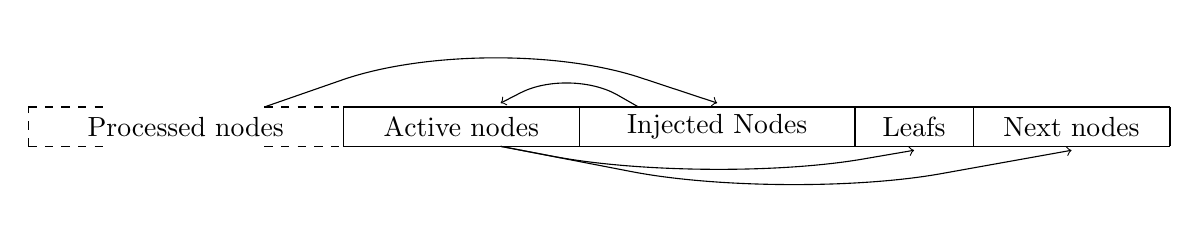
\begin{tikzpicture}[y=0.5cm, x=0.5cm]
    \draw[dashed] (0,1) -- (2,1);
    \draw[dashed] (0,0) -- (0,1);
    \draw[dashed] (0,0) -- (2,0);
    \draw (4,0.5) node {Processed nodes};
    \draw[dashed] (6,1) -- (8,1);
    \draw[dashed] (6,0) -- (8,0);
    \draw (8,1) -- (8,0);

    \draw (8,1) -- (29,1);
    \draw (8,0) -- (29,0);

    \draw (11,0.5) node {Active nodes};
    \draw (14,1) -- (14,0);

    \draw (17.5,0.5) node {Injected Nodes};
    \draw (21,1) -- (21,0);

    \draw (22.5,0.5) node {Leafs};
    \draw (24,1) -- (24,0);

    \draw (26.5,0.5) node {Next nodes};
    \draw (29,1) -- (29,0);

    \draw[rounded corners=20mm, ->] (6,1) -- (11.75, 3) -- (17.5,1.1);
    \draw[rounded corners=7mm, ->] (15.5,1) -- (13.75,2) -- (12,1.1);
    \draw[rounded corners=20mm, ->] (12,0) -- (17.25,-1) -- (22.5,-0.1);
    \draw[rounded corners=20mm, ->] (12,0) -- (19.25,-1.4) -- (26.5,-0.1);

  \end{tikzpicture}
  \caption[The structure of the kd-trees nodes in memory with Empty Space
    Maximization.]{The structure of the kd-trees nodes in memory with Empty
    Space Maximization. The arrows symbolize the parent$\rightarrow$child
    relationship.}
  \label{fig:emptyNodeStructure}
\end{figure}


% Propagating aabb's downwards

With the addresses of the nodes produced by Empty Space Maximization computed, a
kernel can be launched that creates the actual empty space nodes and rewires the
parent node to point to the empty space nodes instead of its current child node.

This construction is very flexible and all computations needed by Empty Space
Maximization can be turned on and off at will, which allows me to easily compare
the quality and construction speed of trees with and without this optimization.

\subsection{Lower Tree Creation}\label{sec:lowerNodes}

Compared with the upper tree creation phase, the lower tree creation is quite
simple and only requires a few kernels. Since there can be thousands of active
nodes at the lower node phase, parallization can effectively be done over nodes
instead of triangles.

\zhou{} proposes that the surface area heuristic is used when deciding which
splitting candidate to use and that the set of splitting candidates is
precomputed from the geometry's bounding volumes. Precomputing the splitting
candidates instead of adjusting them after each split, can cause SAH to not
choose the most desireable splitting plane. This has already been discussed in
\refsection{sec:SAH} in the Split Candidates paragraph and
\vreffig{fig:aabbSplit} presents an example. \zhou's reasoning for doing it
anyway is

\quotebook{While clipping is effective for large nodes by preventing false
  postives from accumulating over future splits, our experiments indicate that
  clipping rarely improves ray tracing performance.}{1409079}

%\fixme{This means?}

%% Later in this section I will propose two simplifications to the standard SAH
%% approach. These simplifications may both produce acceleration structures of
%% lower quality than the computationally heavy SAH, but they make up for this
%% by being much faster.

\subsubsection{Lower Tree Split Candidates}

% Explain the Plane struct

%\fixme{Explain that this amounts to box inclusion?}

Before splitting any nodes however, I first introduce the split candidate
structure used in the lower node phase. Recall from
\refsection{sec:treeRepresentation} that a node stores the reference to its
associated triangles as an index, $i$, and a range, $r$, into the list of all
triangles. To efficiently compute the number of triangle associated with a node
and performing triangle/node association in one instruction, I adopt \zhou's
novel approach of storing a node's triangle association using an index, $i$, and
a bit mask, $b$. If the $k$'th bit in $b$ is set, this means that the $i+k$'th
triangle in the list of all triangles is associated with the node. The bit mask
corrosponding to $r$ would then simply have all its first $r$ bits set. A more
thorough example of how bit masks are used is given in \reffig{fig:bitmap}.

%\fixme{Better explanation of how planes are precomputed and used, example!}

\newcommand{\nodeBitmap}[5]{
  \begin{tabular}{c}
    #1 \\ 
    \begin{tikzpicture}[y=0.4cm, x=.4cm,font=\sffamily]
      \draw (0,0) -- (4,0);
      \draw (0,1) -- (4,1);
      \draw (0,0) -- (0,1);
      \draw (1,0) -- (1,1);
      \draw (2,0) -- (2,1);
      \draw (3,0) -- (3,1);
      \draw (4,0) -- (4,1);
      
      #2
      #3
      #4
      #5
    \end{tikzpicture}
  \end{tabular}
}

\begin{figure}
  \centering
  \subfloat[]{
    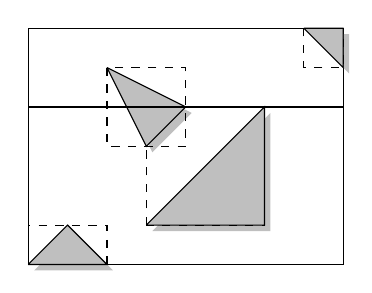
\begin{tikzpicture}[y=0.5cm, x=.5cm,font=\sffamily]
      \draw (0,0) -- (0,6) -- (8,6) -- (8,0) -- (0,0);

      \drawTri{0,0}{2,0}{1,1}
      \drawAabb{0,0}{0,1}{2,1}{2,0}
      \drawTri{3,1}{6,1}{6,4}
      \drawAabb{3,1}{3,4}{6,4}{6,1}
      \drawTri{7,6}{8,6}{8,5}
      \drawAabb{7,6}{8,6}{8,5}{7,5}
      \drawTri{2,5}{3,3}{4,4}
      \drawAabb{2,5}{2,3}{4,3}{4,5}

      \draw (0,4) -- (8,4);
    \end{tikzpicture}
  }
  \subfloat[]{
    \begin{tikzpicture}[y=0.5cm, x=.5cm,font=\sffamily,
        level/.style={sibling distance=50mm/#1}]
      \node [node] {\nodeBitmap{0}
        {\drawTri{0.2,0.3}{0.5,0.6}{0.8,0.3}}
        {\drawTri{1.2, 0.8}{1.5, 0.2}{1.8, 0.5}}
        {\drawTri{2.2,0.2}{2.8,0.2}{2.8,0.8}}
        {\drawTri{3.2, 0.8}{3.8, 0.8}{3.8, 0.2}}}
      child {node [leaf] {\nodeBitmap{1}
          {\drawTri{0.2,0.3}{0.5,0.6}{0.8,0.3}}
          {\drawTri{1.2, 0.8}{1.5, 0.2}{1.8, 0.5}}
          {\drawTri{2.2,0.2}{2.8,0.2}{2.8,0.8}}{}}}
      child {node [leaf] {\nodeBitmap{2}{}
          {\drawTri{1.2, 0.8}{1.5, 0.2}{1.8, 0.5}}{}
          {\drawTri{3.2, 0.8}{3.8, 0.8}{3.8, 0.2}}}};
    \end{tikzpicture}
  }
  \caption[A description of storing triangles as bit masks.]{A description of
    storing triangles as bit masks. The bit masks are represented by a grid
    containing the triangles. If a grid cell contains a triangle, then that bit
    is set. Node 0 contains all triangles, as evidenced by its bit mask. Node 0
    is then split along the precomputed split candidate drawn in the scene,
    which has the left triangle bit mask $[1,1,1,0]$ and right mask
    $[0,1,0,1]$. The result of splitting is leafs 1 and 2, whose triangle bit
    masks are the result of a bitwise \textbf{AND} between node 0's bit mask and
    the split candidate's left and right bit mask respectively.}
  \label{fig:bitmap}
\end{figure}

% Example of how to store splitting planes as bitmasks

Since the split candidates are local to the lower subtree, they too benefit from
the bit mask representation. Each split candidate needs to store two triangle
bit masks, the triangles in front of the splitting plane and the triangles
behind. The method for computing the triangle bit masks of the precomputed split
cnadidates can be seen in \refalg{alg:calcSplittingPlanes}, which only computes
them along the x-axis, but is trivially extended to other dimensions. The
algorithm uses a triangle's axis aligned bounding box, $aabb_t$ to determine on
which side of the splitting plane the triangle is located. If $aabb_t$'s minimum
cornor is in front of the splitting plane, then the $t$'th bit in the triangle
bit mask in front of the plane is set. If the maximum cornor of $aabb_t$ is
behind the plane, then the triangle bit mask for the triangles behind the plane
will have its $t$'th bit set.

% Using shared memory

\Refalg{alg:calcSplittingPlanes} loops over the list of triangles twice, once in
parallel and once for each thread. This results in a lot of global memory
access, which can potentially slow down the procedure. This is optimized the
same way as in \refsection{sec:usingSharedMem}, where the threads in a warp
worked together to load data into shared memory and then accessed that instead
of global memory. To better convey the intent of
\refalg{alg:calcSplittingPlanes} this optimization has been left out.



With the split candidates precomputed and their left and right triangle sets
stored as bit masks, it becomes trivial to associate a triangle with a child
node after a split. E.g. a new left child's triangle bit mask would simply be
the bitwise \textbf{AND} of its parent's bit mask and the bit mask for the
triangle set in front of the splitting plane. \Reffig{fig:bitmap} also gives an
example of this, as Node 0 is split by a splitting plane with the triangle bit
mask $[1,1,1,0]$ in front and $[0,1,0,1]$ behind. Hereafter the triangle bit
mask in front of a split candidate will be refered to as its left triangle bit
mask and the bit mask behind is its right.

\begin{algorithm}
  \caption{Preprocess Lower Nodes.}
  \label{alg:calcSplittingPlanes}
  \begin{algorithmic}
    \PROCEDURE{PreprocessLowerNodes}
              {$upperLeafs$ : Node List}
              {}{
                \PARALLELFOR{$node$}{$upperLeafs$}
                  \PARALLELFOR{$triangle$}{$node.Triangles$}
                    \ASSIGN{$aabb_p$}{GetAabb($triangle$)}
                    \COMMENTIT{Create the splitting plane sets along the x-axis.}
                    \DECLARE{$x_{low}, x_{high}$}{Plane}
                    \FOREACH{$t$}{$node.Triangles$}
                      \ASSIGN{$aabb_t$}{GetAabb($t$)}
                      \ASSIGN{$x_{low}.left[t]$}{$aabb_t.min.x <= aabb_p.min.x$}
                      \ASSIGN{$x_{low}.right[t]$}{$aabb_p.min.x < aabb_t.max.x$}
                      \ASSIGN{$x_{high}.left[t]$}{$aabb_t.min.x <= aabb_p.max.x$}
                      \ASSIGN{$x_{high}.right[t]$}{$aabb_p.max.x < aabb_t.max.x$}
                    \ENDFOR
                    \STATE{$node.splitCandidates$.Add($x_{low}$)}
                    \STATE{$node.splitCandidates$.Add($x_{high}$)}
                    \STATE{...}
                    \COMMENTIT{Perform similar plane constructions for the y and z axis.}
                    \STATE{...}
                  \ENDFOR
                \ENDFOR
              }
  \end{algorithmic}
\end{algorithm}



\subsubsection{SAH Tree Construction}

% Adds surface area computation to the preprocess

With the splitting planes defined and computed, it is now possible to split the
nodes. \zhou{} used SAH to chose a splitting plane, so this will also be our
first approach. While SAH did not fit the upper tree construction phase because
of too many triangles per node and the assumption that all splits resulted in
leaf nodes, these are the very reasons that it fits so much better for lower
tree construction. As noted previously in \refsection{sec:kdTreeImpl},
lower trees are constructed from leaf nodes maximally referencing 32 or 64
triangles. This means the time complexity for computing $C_{SAH}$ per node is
now bounded by $O(32^2) = O(1)$ or $O(64^2) = O(1)$, instead of $O(t^2)$ in the
upper tree phase, where $t$ is the number of triangles in an upper node and can
be hundreds of thousands. Also the assumption that a split will result in two
leafs in the final tree is far more likely to be true at the lower tree phase
than the upper phase.

\begin{algorithm}
  \caption{Calculate SAH cost}
  \label{alg:calcSAHCost}
  \begin{algorithmic}
    \PROCEDURE{ComputeSAHCost}
              {$activeNodes$ : Node List}
              {$splittingPlanes$ : Plane List, $leafs$ : Boolean List}{
                \COMMENTIT{Calculate SAH cost for each split candidate and
                  return the split candidate with minimal cost.}
                \PARALLELFOR{$node$}{$activeNodes$}
                  \FOREACH{$candidate$}{$node.splitCandidates$}
                    \ASSIGN{$set_l$}{$node.triangles \cap candidate.left$}
                    \ASSIGN{$C_l$}{$\parallel set_l \parallel$}
                    \ASSIGN{$A_l$}{summed surface area of $set_l$}
                    \ASSIGN{$set_r$}{$node.triangles \cap candidate.right$}
                    \ASSIGN{$C_r$}{$\parallel set_r \parallel$}
                    \ASSIGN{$A_r$}{summed surface area of $set_r$}
                    \ASSIGN{$weightedArea$}{$C_l \cdot A_l + C_r \cdot A_r$}
                  \ENDFOR
                  \ASSIGN{$splittingPlanes[node] \leftarrow p$}{Split candidate with minimal weighted area}
                  \ASSIGN{$C_{SAH}$}{$C_{trav} + p.weightedArea / node.summedArea$}
                  \ASSIGN{$leafs[node]$}{$C_{SAH} < C_{leaf}$}
                \ENDFOR
              }
  \end{algorithmic}
\end{algorithm}

% Explain

The algorithm for computing the SAH cost of a splitting plane is given in
\refalg{alg:calcSAHCost}. As described earlier the algorithm is parallelized
over all nodes. A node must then iterate over all useful split candidates,
i.e. those split candidates that were created from bounding boxes of the node's
triangles. For each split candidate the weighted area, $C_l \cdot A_l + C_r
\cdot A_r$, is computed and the one with the lowest is stored as the proposed
splitting plane. The SAH value of the best split candidate is then computed and
compared to the cost of leaving the node as a leaf node. The result of this
comparison is returned at the end of the algorithm along with the best splitting
plane.

% Run prefix sum on leafList and use the result as addresses for the
% children.

A kernel then creates children to the nodes where $SAH < C_{leaf}$. In order to
do this however, we must again first apply the prefix-sum. This time we apply it
to the $leafs$ list and use the result to find the addresses where a nodes
children should be created. An example is given below, where nodes $n_0$ and
$n_2$ should have leafs created and these should be created at address 0 and 2
respectively.

\begin{displaymath}
  \begin{array}{r c c c c l}
    node: & [n_0 & n_1 & n_2 & n_3]\\
    leafs: & [1 & 0 & 1 & 0]\\
    prefix\text{-}sum: & [0 & 1 & 1 & 2]\\
    address: & [0 & 2 & 2 & 4] & // prefix\text{-}sum \cdot children\text{ }per\text{ } node\\
  \end{array}
\end{displaymath}



\subsubsection{Simplified SAH Tree Construction}

% SAH is slow, so explore alternatives.

While SAH's time complexity per node is $O(1)$, the iteration over all triangles
assocated with a node to compute $A_l$ and $A_r$ is still quite expensive. For
dynamic scenes I propose the following simplifying assumptions: That all
triangles have the same surface area, specifically the surface area
1. Calculating $A_n$ for a given node $n$ could then be reduced from a loop to
one single instruction $A_n = \|set_n\|$ and the entire SAH cost computation can
be simplified as follows.

\begin{displaymath}
  \begin{array}{r l}
    & C_{SAH}(n \rightarrow \{l, r\}) = C_{trav} + \frac{C_l A_l}{A_n} + \frac{C_r
      A_r}{A_n}\\
    \Downarrow \\
    & C_{SSAH}(n \rightarrow \{l, r\}) = C_{trav} +
    \frac{C_i \|set_l\|^2}{\|set_n\|} + \frac{C_i \|set_r\|^2}{\|set_n\|}\\
  \end{array}
\end{displaymath}

% Introducing the simplified SAH split.

\begin{algorithm}
  \caption{Calculate simplified SAH cost}
  \label{alg:calcBalancedCost}
  \begin{algorithmic}
    \PROCEDURE{ComputeSimpleSAH}
              {$activeNodes$ : Node List}
              {$splittingPlanes$ : Plane List, $leafs$ : Boolean List}{
                \COMMENTIT{Calculate the simplified SAH cost for each split candidate and
                  return the split candidate with minimal cost.}
                \PARALLELFOR{$node$}{$activeList$}
                  \ASSIGN{$p$}{$noSplitCandidate$}
                  \FOREACH{$candidate$}{$node.splitCandidates$}
                    \ASSIGN{$set_l$}{$node.triangles \cap candidate.left$}
                    \ASSIGN{$set_r$}{$node.triangles \cap candidate.right$}
                    \ASSIGN{$weightedArea$}{$\|set_l\|^2 + \|set_r\|^2$}
                  \ENDFOR
                  \ASSIGN{$splittingPlanes[node] \leftarrow p$}{Split candidate with minimal weighted area}
                  \ASSIGN{$C_{SSAH}$}{$C_{trav} + p.weightedArea / \|node.triangles\|$}
                  \ASSIGN{$leafs[node]$}{$C_{SSAH} < C_{leaf}$}
                \ENDFOR
              }
  \end{algorithmic}
\end{algorithm}

% Explain

The algorithm for computing this \textit{Simplified Surface Area Heuristic} or
\textit{SSAH} can be seen in \refalg{alg:calcBalancedCost} and works similarly
to \refalg{alg:calcSAHCost}. Just as with the SAH approach, child nodes are
created in a seperat kernel after prefix-sum has been applied to the list
$leafs$.

\subsubsection{No Tree Construction}

The final tree construction algorithm I will propose for the lower tree phase is
extremely simple: Do not create any tree!

Recall from \refsection{sec:memoryModel} that the latency of global memory
access becomes harder for the multiprocessor to hide if threads' global memory
access can not be coalesced. This can happen for threads in the same warp
traversing a tree, since at some point they are likely to diverge and traverse
different parts of the tree, which results in scattered global memory
accesses. Favoring leaf nodes with more triangles associated would reduce the
size of the tree and thus the thread divergence. Reducing thread divergence
would then in turn allow the warp to better coalesce global memory access and
thereby reducing memory transaction and easier hide memory latency. I therefore
propose not to create a lower tree, but instead terminate after having created
the upper tree. This would save both the time spent preprocessing the nodes to
compile the list of split candidates and the time spent actually creating the
subtree.

Which of the lower tree construction methods proves the best will be evaluated
in \refsection{sec:evaluateLowerTree}.


\chapter{Ray Tracing}

\chapterquote{Some argue that in the very long term, rendering may
  best be solved by some variant of ray tracing, in which huge numbers
  of rays sample the environment for the eye’s view of each frame. And
  there will also be colonies on Mars, underwater cities, and personal
  jet packs.}{Tomas Möller and Eric Haines}

% Motivate!

% We will build an exhaustive ray tracer to test the quality of the kD
% tree.

% An optimized ray tracer will be used to test wether or not more time
% spend on creating a better kD tree will pay off in final rendering
% time.

% Optimizations will be added incrementally to the hierarchical ray
% tracer and implementation details to each specific optimization will
% therefore be discussed alongside the theory.

The optimized ray tracer will use techniques from \citebook{Aila2009}
and \citebook{1230129}.

\section{Triangle Intersection}

% Consists of 2 parts. Ray/plane intersection which tells us the
% distance the ray will travel, and ray/triangle tests which tells us
% if the ray intersected the triangle.

% Explain barycentric coordinates and how they are important for
% triangle/ray intersection and linearly interpolating the triangle
% attributes at the vertices, such as the normals, colors or texture
% coordiantes. Convex combination?

% Use the barycentric coordinates to perform the intersection test.
For a barycentric coordinate to be inside the triangle it must fulfill
$0 \le u$, $0 \le v$ and $u+v \le 1$.

\subsection{Möller-Trumbore}

% One of the most popular intersection algorithms and featured in
% Real-Time Rendering.

The Möller-Trumbore algorithm presented in \citebook{MollerTrumbore97}
is one of the most popular algorithms for ray/triangle intersection,
due probably in no small part to it's appearence in chapter 16.8 in
\citebook{RTR3}, but also because it is one of the fastest
ray/triangle intersection algorithms that does not rely on extra
memory and/or precomputation.

% Computes both distance and barycentric coords

% Calculates the transformation that transform the triangle into the
% unit triangle and applies this transformation to the ray.

The basic idea of their algorithm is to find the affine transformation
that when applied to the triangle, $T(u,v)$, given by

\begin{displaymath}
  T(u,v) = (1-u-v)a + ub + vc
\end{displaymath}

transforms it into the unit triangle, $U$, which has vertices
$\vecthreeT{0}{0}{0}$, $\vecthreeT{1}{0}{0}$ and
$\vecthreeT{0}{1}{0}$. That affine transformation is then instead
applied to the ray, $R(t) = o + td$, which yields the vector
$\vecthreeT{t}{u}{v}$, where $t$ is the distance to the plane spanned
by $T(u,v)$ and $u$ and $v$ are the barycentric coordinates of the
intersection point.

In short this boils down to solving the linear system of equations

\begin{displaymath}
  \begin{array}{rl}
    & R(t) = T(u,v) \\
    \Updownarrow \\
    & o + td = (1-u-v)a + ub + vc \\
  \end{array}
\end{displaymath}

As can be seen in \citebook{MollerTrumbore97}, by rearranging the
terms and applying Cramer's Rule, the solution is

\begin{displaymath}
  \vecthree{t}{u}{v} = \frac{1}{P \cdot E_1} 
  \vecthree{Q \cdot E_2}{P \cdot T}{Q \cdot D}
\end{displaymath}

where $E_1 = b - a$, $E_2 = c - a$, $T = o - a$, $P = d \times  E_2$
and $Q = T \times  E_1$.

\subsubsection{Implementation}

% Due to the GPU's SIMT architecture, providing as many early out
% possiblities as Möller-Trumbore's implementation caused a branching
% overhead. The universal sweetspot in all of this thesis ray tracers
% was found to be ...

\subsection{Woop}

% Also translates the ray using the unit triangle.

As was the case with the Möller-Trumbore approach, Woops was also
interested in transforming the generel ray/triangle intersection
problem into a ray/unit triangle intersection problem, where the
solution is trivially calculated.

He observed that the triangle, $T$, can be transformed into the unit
triangle, $U$, via an affine transformation, consiting of a rotation
matrix, $m$, and a translation, $n$.

\begin{displaymath}
  U_d = m T_d + n, d \in \{x, y, z\}
\end{displaymath}

% Does some precalculation, which means we can save calculations and
% register space when performaing the actual ray tracing.

% The extra space used by the precalcultations can be mitigated if
% the vertices are no longer needed.

\subsubsection{Implementation}

% Higher occupancy, which in turn will make it easier for the GPU to
% hide global memory lookup latency. Or not. Still at 32 registers.




\section{Exhaustive Ray Tracing}

% GPU does bruteforcing well.

% Cite paper on kNN done on the GPU.

% Algorithm

% GPU optimazations? Can shared mem work damn it?!?

\section{Hierarchical Ray Tracing}

% Brief introduction to several acceleration techniques. BVH, KD,
% quad/oct trees and BSP.

% KD-trees are ze leetzors according to Havran? Another motivation is
% Zhou's paper on fast KD tree construction.

\subsection{KD-restart}

% KD restart is the simplest and fastest.

% Start with kd restart, simple to get up and running.

\begin{algorithm}
  \caption{KD Restart}
  \label{alg:KDRestart}
  \begin{algorithmic}
    \PROCEDURE{KDRestart}
              {$ray$ : Ray}
              {$t_{min}$ : Integer}{
                \ASSIGN{$t_{min}$}{$0$}
                \WHILE{$t_{min} < \infty$}
                  \ASSIGN{$t_{next}$}{$\infty$}
                  \ASSIGN{$node$}{$root$}
                  \COMMENTIT{Traverse the tree until a leaf node is reached}
                  \WHILE{$node.info \neq LEAF$}
                    \ASSIGN{$t_{split}$}{($node.splitValue - ray.origin[node.axis]) / ray.direction[node.axis]$}
                    \IF{$t_{min} < t_{split}$}
                      \ASSIGN{$node$}{$ray.direction[node.axis] > 0$ ? $node.left$ : $node.right$}
                      \ASSIGN{$t_{next}$}{min$(t_{split}, t_{next})$}
                    \ELSE
                      \ASSIGN{$node$}{$ray.direction[node.axis] > 0$ ? $node.right$ : $node.left$}
                    \ENDIF
                  \ENDWHILE
                  \COMMENTIT{Advance the ray to the next splitting plane.}
                  \ASSIGN{$t_{min}$}{$t_{next}$}
                  \COMMENTIT{Test intersection with the leafs primitives}
                  \FOREACH{$triangle$}{$node.triangles$}
                    \ASSIGN{$t_{min}$}{min$(t_{min}, $\bf{Intersect}$(triangle, ray))$}
                  \ENDFOR
                \ENDWHILE
                \STATE{\bf{return} $t_{min}$}
              }
  \end{algorithmic}
\end{algorithm}

\subsection{Packets}

% Packets: 2x2 packets on the CPU for to take advantage of SIMD
% instructions (Wald), warp size packets on the GPU. While
% \citebook{1230129} implemented packets, they merely assumed it would
% yield a speedup and did not provide any results. Aila2009 is against
% packets as they in practice seem to make it slower.

% As ray tracing becomes more complex packets also become less
% effective, as rays will become more chaotic in nature and less
% likely to fit into packets.

% I will adobt a pretty cheap packet strategy: I will trace my rays in
% 4x8 packets to increase ray coherence across warps.

\subsection{Short stack}

% Only push usefull 'forward' nodes to the stack.

\begin{algorithm}
  \caption{Short stack}
  \label{alg:ShortStack}
  \begin{algorithmic}
    \PROCEDURE{ShortStack}
              {$ray$ : Ray}
              {$t_{min}$ : Integer}{
    \ASSIGN{$t_{min}$}{$0$}
    \WHILE{$t_{min} < \infty$}
      \IF{$\color{green}stack.IsEmpty$}
        \ASSIGN{$node$}{$root$}
        \ASSIGN{$t_{next}$}{$\infty$}
      \ELSE
        \color{green}\ASSIGN{$(node, t_{next})$}{stack.pop}
      \ENDIF
      \COMMENTIT{Traverse the tree until a leaf node is reached}
      \WHILE{$node.info \neq LEAF$}
        \ASSIGN{$t_{split}$}{($node.splitValue - ray.origin[node.axis]) / ray.direction[node.axis]$}
        \IF{$t_{min} < t_{split}$}
          \ASSIGN{$node$}{$ray.direction[node.axis] > 0$ ? $node.left$ : $node.right$}
          \IF{$\color{green}t_{split} < t_{next}$}
            \color{green}\STATE{stack.push($upperChild, t_{next}$)}
          \ENDIF
          \ASSIGN{$t_{next}$}{min$(t_{split}, t_{next})$}
        \ELSE
          \ASSIGN{$node$}{$ray.direction[node.axis] > 0$ ? $node.right$ : $node.left$}
        \ENDIF
      \ENDWHILE
      \COMMENTIT{Advance the ray to the next splitting plane.}
      \ASSIGN{$t_{min}$}{$t_{next}$}
      \COMMENTIT{Test intersection with the leafs primitives}
      \FOREACH{$triangle$}{$node.triangles$}
        \ASSIGN{$t_{min}$}{min$(t_{min}, $\bf{Intersect}$(triangle, ray))$}
      \ENDFOR
    \ENDWHILE
    \STATE{\bf{return} $t_{min}$}
              }
  \end{algorithmic}
\end{algorithm}

\subsection{Push Down}

I will not be implementing the push-down approach from
\citebook{1230129}. While it will most likely improve the generel ray
tracing case, where some of the geometry will be located behind the
rays and can safely be excluded, it will only add an overhead to worst
case situations, where the uppermost splitting plane is intersected by
the rays.

\subsection{Ropes}

% stackless raytracing using ropes. 
% Place in future works?

\subsection{Persistent Threads}

% Use persistent threads / own scheduler. Aila2009.

\subsection{Caching 'hot' nodes}

% wrap node and geometry arrays in textures to utilize cache? Or
% simply don't care and refere to cached global memory in future
% GPU's?

% Like persistent threads, this is not an important optimazition
% longterm, since global memory are being given a cache.



\section{Coloring}

% Everything is paper thin and empty space


% -*- mode: latex; mode: auto-fill; coding: utf-8; -*-

\chapter{Results}

\chapterquote{It’s hardware that makes a machine fast. It’s software
  that makes a fast machine slow.}{Craig Bruce}

% Tabels of nodes and triangled visited. Perhaps some statistics over
% wasted iterations by threads waiting for other threads in the warp
% to finish. The high triangle count pr leaf optimization may be
% related to this and makes using highly optimized splitting plane
% calculations in the lower nodes useless.

\chapter{Conclusion}

\chapterquote{The best thing about a boolean is even if you are wrong,
  you are only off by a bit.}{Anonymous}

\chapter{Future Work}

\chapterquote{Software is like entropy: It is difficult to grasp,
  weighs nothing, and obeys the Second Law of Thermodynamics; i.e., it
  always increases.}{Norman Augustine}

Look at stackless raytracers with ropes.

Using Morton Keys for data structure creation.

Photon Mapping. Which simplifies a lot of the kd tree creation by not
requiring splits.



\newpage
\phantomsection \label{bib}
\addcontentsline{toc}{chapter}{Bibliography}
\bibliographystyle{amsplain}
\bibliography{refs}

\newpage
\phantomsection \label{listofalg}
\addcontentsline{toc}{chapter}{List of Algorithms}
\listofalgorithms

\newpage
\phantomsection \label{listoffig}
\addcontentsline{toc}{chapter}{List of Figures}
\listoffigures

\appendix

\chapter{Uptaining the source}

This project has been developed in OpenEngine, which is needed to
uptain the source code.

A guide for installing OpenEngine can be found at
\url{http://www.openengine.dk/trac/wiki/Download}.

\fixme{Write this!}


%
\section*{Road Map}


\begin{itemize}
\item \color{green}Create the KD-tree from points on the GPU \checkmark
\item Visualize the KD-tree (as part of debugging), draw frame around
  splitting plane in color corrosponding to splitting axis. (\checkmark)
\item Extend KD-tree to work on triangles \checkmark
\item raytrace the triangle KD-tree \checkmark
\item Add a balanced tree lower node creator \checkmark
\item Reduce more than 1024 segments \checkmark
\item Add empty space splitting
  \begin{itemize}
    \item Extend CreateUpperChildren with the possibility to use indices \checkmark
    \item Copy aabb to lower nodes \checkmark
    \item In reduce, compare the existing aabb with the reduced. \checkmark
    \item Move the nodes by the amount of emptySplitNodes, create the
      empty split nodes in front of the nodes and link them with the
      previous nodes parents.\\ Remember to update segments (used when
      splitting triangles), node size and activeIndex. \checkmark
    \item \color{red}Make dynamic empty space threshold. Higher probability of
      splits at the top, than bottom.
    \item PROFIT
  \end{itemize}
\item Optimize GeometryList
  \begin{itemize}
  \item Removed OpenGL and use device arrays instead. Oh such clean
    geometry collection code. \checkmark
  \end{itemize}
\item Partition the screen into 8x4 ray blocks to improve ray
  traversel coalescenece. \checkmark
\item Use triangle-box intersection to remove ``impossible to hit''
  triangles from the lower nodes. Aabb might need to be propagated
  downwards in order to do this.
\item Create an optimized aabb intersection algorithm that
optimizes with respect to a triangle and 2 boxes. Doesn't work due to
the compiler dropping the ball when switches contain huge cases..
\item Use woop triangle intersection instead while raytracing (Make an
  enum that can switch). Place the offset in the fourth component of
  each vector, that way I only need to load 1 float4 pr tHit
  component. Less register usage! Yielded 20\% increase on dragon2 in
  cornell box.
\item Make colors float instead of char. Removes 4 divisions when
  coloring. (And apparently add a data fetching overhead, not worth
  it)
\item Add a bounding box check before raytracing leafs? Provides an
  early out option for long rays. Nice speedup. Won't work aswell with
  small leaf nodes? Inspired by empty space splitting.
\item Instead of moving nodes when doing an empty split, place them
  empty nodes after index + range and remember to skip them when
  creating children. (node size can be used for this, and the
  outermost while loop works unaltered).

\color{red}
\item Make indices in primMin and tHit a float\_to\_int gøjler. Saves
  an actual conversion (and like what, 2ms total, boy you're starting
  to go overboard here)
\item Instead of resizing aabbs, perhaps just use the original size
  and crop it with the propagated aabb. Then test if splitting and
  creating new aabbs even adds any speed or if indexing is faster.
\item Add triangle split. Triangle split can possibly gain
  some performance, by always doing the ``2 triangles'' side first.
\item Perhaps node creation can be sped up by adding a shared mem
  block cache and then dumping data coallesced.
\item Fix KernelConf1D when registers are used (something about 512bit
  allocation, unless 2.0 architeture)
\end{itemize}

If time allows

\begin{itemize}
\item Store empty split nodes in shared mem and then dump it all
  coallesced after they have been created.
\item Speed up node child creation by using shared mem as
  cache. Enough threads to fill the GPU could be started and then each
  work on their continous segment of the nodes
\item Speedup shadow rays and ambient occlusion. Mostly from simpler
  intersection testing and less register usage.\\ -- OR -- \\ Perhaps
  let the primary raytracer to it's job (coloring and refraction),
  then dump the individual colors and primitive indices into arrays
  (some MAX like 5?), let a different raytracer pickup these values
  and start tracing shadows. Combine everything in a last kernel for
  PROFIT.
\item Add Persistent Theads to SAH. Extend it with preemtively
  replacing dead threads every 4 or so cycle.
\item Add persistent threads to the ray tracer
\item Add an oscilating surface with nice refraction!!
\item Look into SAH approximations
\item At lower tree levels where SAH isn't computed parallel, perhaps
  and early out ``good enough'' value/ratio can be given, as done in
  BSP. Might only increase instructions, branching and still wait for
  the slowest thread. (Try and watch it fail) Perhaps without an if
  statement but by arithmetic instead?
\item Perhaps empty space splitting can be started in it's own stream?
  At least the actual empty space splitting should be able to. Could
  help out at the early tree creation when the GPU is
  underutilized. Suggest or actually try? Would make it an even
  cheaper optimization.
\item Optimize segmented reduce. (low low priority)
\end{itemize}




\subsection*{Sangild}

Bank conflicts.

====

Occupancy

Primære og sekundære kilder? Both good. Just quote responsibly (page
number, section, something)

Slå register usage op på runtime? Can't be done. Hardcode the
bastards. And fix KernelConf1D when registers are used (something
about 512bit allocation, unless 2.0 architeture)


\end{document}
